% File that compiles all other files into one clean document.

%Layout, imports, packages, class
%%%%%%%%%%%%%%%%%%%%%%%%%%%%%%%%%%%%%%%%%%%%%%%%%%
% PAGE LAYOUT
%%%%%%%%%%%%%%%%%%%%%%%%%%%%%%%%%%%%%%%%%%%%%%%%%%
\documentclass[a4paper,11pt]{report}
%\usepackage[subtle]{savetrees}
\usepackage{fullpage}
\usepackage{wrapfig}
%%%%%%%%%%%%%%%%%%%%%%%%%%%%%%%%%%%%%%%%%%%%%%%%%%
%% PAGEHEADER STYLING
%%%%%%%%%%%%%%%%%%%%%%%%%%%%%%%%%%%%%%%%%%%%%%%%%%
\usepackage{etoolbox,fancyhdr,xcolor}
%%%%%%%%%%%%%%%%%%%%%%%%%%%%%%%%%%%%%%%%%%%%%%%%%%
% EXTERNAL INCLUDES
%%%%%%%%%%%%%%%%%%%%%%%%%%%%%%%%%%%%%%%%%%%%%%%%%%
\usepackage{graphicx}
\usepackage{svg}
\usepackage{csvsimple}
\usepackage{pdfpages}
\usepackage{hyperref}
\usepackage{lscape}
\usepackage{eurosym}
%%%%%%%%%%%%%%%%%%%%%%%%%%%%%%%%%%%%%%%%%%%%%%%%%%
%% BIBLIOGRAPHY SETTINGS
%%%%%%%%%%%%%%%%%%%%%%%%%%%%%%%%%%%%%%%%%%%%%%%%%%
\usepackage[comma]{natbib}
\usepackage{color, colortbl}
\usepackage[nonumberlist,acronym]{glossaries}
%%%%%%%%%%%%%%%%%%%%%%%%%%%%%%%%%%%%%%%%%%%%%%%%%%
% CAPTIONS AND REFERENCING
%%%%%%%%%%%%%%%%%%%%%%%%%%%%%%%%%%%%%%%%%%%%%%%%%%
\usepackage{fancyref}
%\usepackage{image_captioning}
%%%%%%%%%%%%%%%%%%%%%%%%%%%%%%%%%%%%%%%%%%%%%%%%%%
%% CODE SNIPPET LISTING SETTINGS
%%%%%%%%%%%%%%%%%%%%%%%%%%%%%%%%%%%%%%%%%%%%%%%%%%
\usepackage{listings}
\renewcommand\lstlistlistingname{List of Listings}
\lstset{numbers=left,xleftmargin=2em,captionpos=b}
%%%%%%%%%%%%%%%%%%%%%%%%%%%%%%%%%%%%%%%%%%%%%%%%%%
%    SECTIONS
%%%%%%%%%%%%%%%%%%%%%%%%%%%%%%%%%%%%%%%%%%%%%%%%%%
\usepackage{titlesec}
\usepackage{sectsty}
\usepackage{csquotes}
%%%%%%%%%%%%%%%%%%%%%%%%%%%%%%%%%%%%%%%%%%%%%%%%%%
%% APPENDIX SETTINGS
%%%%%%%%%%%%%%%%%%%%%%%%%%%%%%%%%%%%%%%%%%%%%%%%%%
\usepackage[titletoc]{appendix}
%\renewcommand\appendixtocname{Appendices}
%\renewcommand\appendixpagename{Appendices}
%All non-canonical parts/chapters should be numbered with roman numbers
\pagenumbering{roman}
\pdfminorversion=7

%Titlepage
\title{Report on Warehouse Drone Collision Avoidance}
\subtitle{Bachelor Thesis}
\author{Tristan van Vegchel}
\date{Venlo, \today}
\requirement{the degree \\ 
	Bachelor of Science in Informatics \\
	To be awarded by the \\
	Fontys Hogeschool Techniek en Logistiek}

%glossaries
\makenoidxglossaries
%File for glossaries

%Glossaries
\newglossaryentry{OpenCV}
{
	name={OpenCV},
	description={OpenCV (Open Source Computer Vision Library) is an open source computer vision and machine learning software library. OpenCV was built to provide a common infrastructure for computer vision applications and to accelerate the use of machine perception in the commercial products. Being a BSD-licensed product, OpenCV makes it easy for businesses to utilize and modify the code} \cite{About_OpenCv}
}

\newglossaryentry{Artificial Intelligence}
{
	name={Artificial Intelligence},
	description={The theory and development of computer systems able to perform tasks normally requiring human intelligence, such as visual perception, speech recognition, decision-making, and translation between languages}
}

\newglossaryentry{deep learning}
{
	name={Deep Learning},
	description={A subset of machine learning in artificial intelligence that makes use of artificial neural networks.}
}

%Abbreviations
\newacronym{STG2}{STG2}{Graduation Project}
\newacronym{AI}{A.I.}{Artificial Intelligence}
\newacronym{FHTenL}{Fontys}{Fontys University of Applied Sciences}
\newacronym{KPI}{KPI}{Key Performance Indicators}
\newacronym{TBD}{TBD}{To Be Determined}
\newacronym{RACI}{RACI matrix}{Responsible-Accountable-Consulted-Informed matrix}
\setacronymstyle{long-short}


%\printnoidxglossary[title=Definitions]

%Bibliography
\renewcommand{\bibname}{References}


%Put includes in document environment
%Wordcount = 556+1022+642+1258+1892+480+374 = 6224
\begin{document}
	\maketitle
	\setcounter{page}{2}
	
	%Information page
	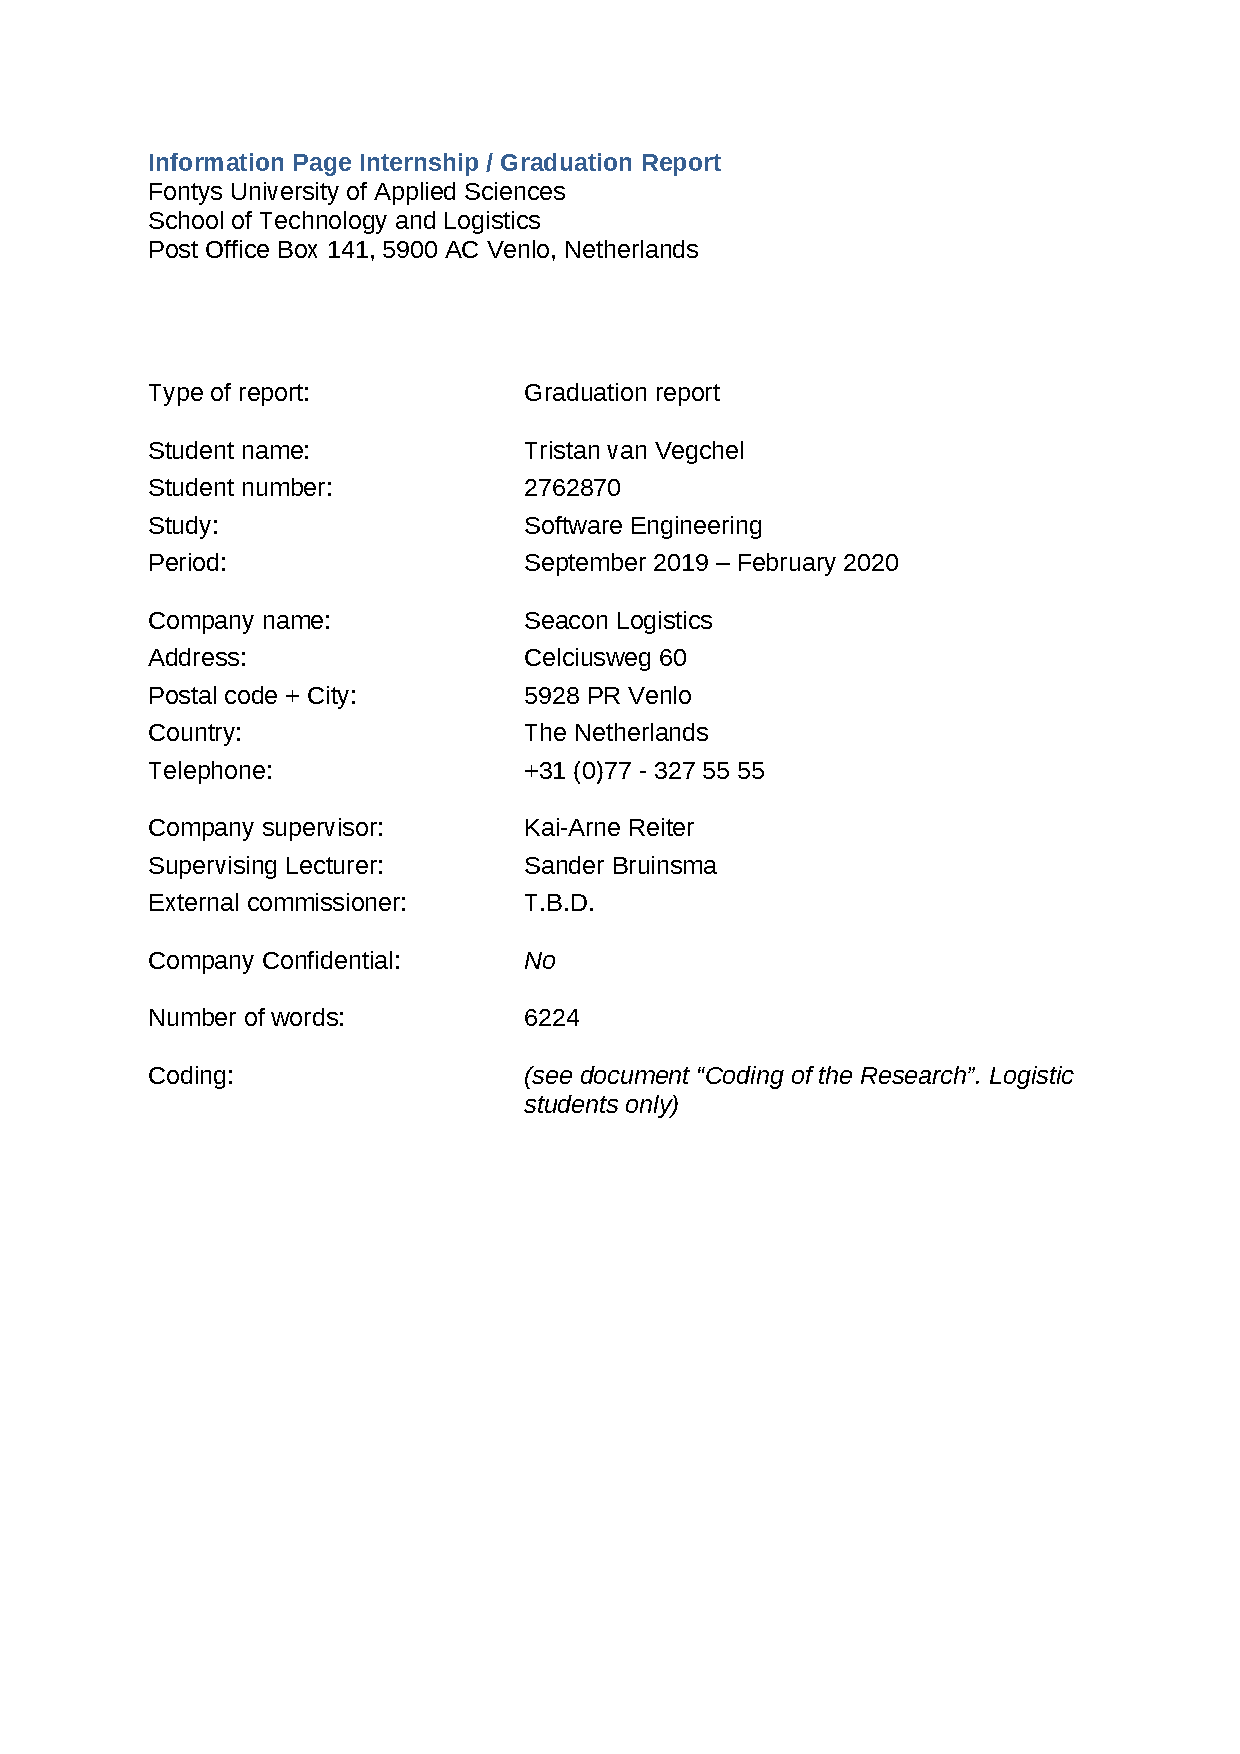
\includepdf[pagecommand={}]{utility/InformationPage}
	
	%Abstract
	\noindent
The warehouse drone collision avoidance project concerns itself with the analysis, design, and development of a solution to provide a drone with collision avoidance functionality. The time scope was set for 1 semester (5 months), and resulted in the creation of this bachelor thesis. This project contains 2 prototype concepts: A concept based on reinforcement learning and a concept based on combining computer vision with a state machine implementation. The reinforcement learning concept did not show promising results as it did not show any sign of learning. The state machine concept its components work separately, but still requires smoother transitioning and a number of bugs needed to be fixed before it is able to run the entire state machine properly. This project also contained a research aspect. This research focused on the viability of Artificial Intelligence techniques for collision avoidance. Out of this came 3 approaches, of which one was created a prototype for. From the research it can be concluded that a single, stand-alone reinforcement learning algorithm is insufficient when attempting to use drones for cycle counting.
	
	%Statement of authenticity
	
\includepdf[pagecommand={}]{utility/Statement_of_Authenticity_new}
	
	%%%%%%%%%%%%%%%%%%%%%%%%%%%%%%%%%%%%%%%%%%%%%%%%%%
%% CONFIGURATION OF PAGE HEADER
%%%%%%%%%%%%%%%%%%%%%%%%%%%%%%%%%%%%%%%%%%%%%%%%%%
\pagestyle{fancy}
\newcommand{\headrulecolor}[1]{\patchcmd{\headrule}{\hrule}{\color{#1}\hrule}{}{}}
\newcommand{\footrulecolor}[1]{\patchcmd{\footrule}{\hrule}{\color{#1}\hrule}{}{}}
\pagestyle{fancy}
\fancyhf{}% Clear header/footer
\fancyhead[C]{}
\fancyhead[R]{\thepage}
\setlength{\headsep}{33pt}
\setlength{\headheight}{13.6pt}
\renewcommand{\headrulewidth}{0.4pt}
\setlength{\parindent}{0em}
	%Content display
	\tableofcontents
	\listoffigures
	\listoftables
	\lstlistoflistings
	
	%Version history
	\pagebreak
	%\vhListAllAuthorsLong
	%Author macros
	\newcommand{\TVV}{Tristan van Vegchel}
	\renewcommand \vhAuthorColWidth{.7\hsize}
	\renewcommand \vhChangeColWidth{1.3\hsize}
	\begin{versionhistory}
		\vhEntry{0.1}{24-10-2019}{\TVV}{Created skeleton}
		\vhEntry{0.2}{15-11-2019}{\TVV}{Added introduction}
		\vhEntry{0.3}{31-12-2019}{\TVV}{Added SRS}
		\vhEntry{0.4}{03-01-2020}{\TVV}{Added approaches}
		\vhEntry{0.5}{06-01-2020}{\TVV}{Added project description}
		\vhEntry{0.6}{08-01-2020}{\TVV}{Added state machine concept}
		\vhEntry{0.7}{09-01-2020}{\TVV}{Updated report after feedback}
		\vhEntry{0.8}{10-01-2020}{\TVV}{Added reinforcement learning concept}
		\vhEntry{0.9}{12-01-2020}{\TVV}{Added conclusion \& recommendations}
		\vhEntry{1.0}{12-01-2020}{\TVV}{Second review and completion of first version}
		\vhEntry{1.1}{13-01-2020}{\TVV}{Consistency changes \& added drone and state descriptions}
		\vhEntry{1.2}{13-01-2020}{\TVV}{Added appendix for installation and setup.}
		\vhEntry{1.3}{13-01-2020}{\TVV}{Grammar changes after third review}
	\end{versionhistory}
	\glsaddall
	\printnoidxglossary[type=\acronymtype,title=List of Abbreviations]
	\printnoidxglossary[title=Definitions]
	
	%Main part
	\pagebreak
	\pagenumbering{arabic}
	
	\chapter{Introduction}
\lhead{\thechapter \space Introduction}
\label{ch:introduction}

\section{Purpose}
%TO DO: Identify the product for which this document is written, as well as the intended audience
The purpose of this document is to provide a detailed description of the software product of the Drone Warehouse Collision Avoidance project. It contains the purpose and features of the software, the interfaces, and the constraints under which it must operate. This document is primarily intended for the department of Engineering \& IT of Seacon Logistics, as this department will contain/contains the future developers of the next iteration of this product. As this project is developed as a bachelor thesis project, the by Fontys University of Applied Sciences appointed tutors, lecturers, and experts are also considered an intended audience.

\section{Document Conventions \& Standards}
%TO DO: Describe any naming or typographical conventions, as well as the standards used (IEEE). For example, state whether priorities  for higher-level requirements are assumed to be inherited by detailed requirements, or whether every requirement statement is to have its own priority.
This document was created based on the IEEE Recommended Practice for Software Requirement Specifications standard 830-1998.

\section{Scope}
%TO DO: Summarize each of the named software products, including what they will and won't do. Also describe the application of the software, such as what the benefits, objectives, and or goals are.
The Warehouse Drone Collision Avoidance system (which is in this document generally referred to as "product") will primarily be responsible for providing a drone with a prototype solution to move along all layers of a single side of a rack in a warehouse, while avoiding collisions.

\section{Overview}
%TODO: List what the rest of this document will contain, and in what order.
The remainder of this document will feature an overall description of the product and the specific requirements. The former includes the perspective, information regarding a set of used interfaces, the product functions, and information regarding the product its users. The latter contains the specific requirements listed with unique identifiers, and a list of assumptions made in order for the product to function.


	\chapter{Project Description}
\lhead{ \thechapter \space Requirements Analysis}
\label{ch:requirements_analysis}
This chapter provides general information regarding the project, and can be considered an introductory chapter of the analysis done. Included is information about stakeholders, the scope, information about the drone, the risks, and a justification. 

\section{Stakeholders \& Affiliates}
Within this project, there are 3 groups of stakeholders: The student, Seacon Logistics, and \gls{FHTenL}. The latter 2 groups shall throughout this document be referred to as either "Seacon" or "the company", and "Fontys" or "the university", respectively. The table below lists individual stakeholders, to which group they belong to, and what their roles are.

\begin{table}[h]
	\centering
	\resizebox{\textwidth}{!}{%
		\begin{tabular}{|l|l|l|l|l|}
			\hline
			\textbf{Name} & \textbf{Company/Institute} & \textbf{Role} & \textbf{RACI Role} & \textbf{Email} \\ \hline
			Tristan van Vegchel & Fontys/Seacon Logistics & Student/Developer & Responsible & Tristan@vanvegchel.eu \\
			Sander Bruinsma & Fontys & Tutor & Informed & S.bruinsma@fontys.nl \\
			Geert Monsieur & Fontys & Examiner & Informed & G.monsieur@fontys.nl \\
			Kai-Arne Reiter & Seacon Logistics & Company Supervisor & Consulted, Informed & Kreiter@seaconlogistics.com \\
			Mark Vromans & Seacon Logistics & Manager Engineering \& IT & Accountable, Informed & Mvromans@seaconlogistics.com \\
			Wilfried Beerens & Seacon Logistics & Manager Shared Services Center & Informed & Wbeerens@seaconlogistics.com \\
			Fred Lemmen & Seacon Logistics & Senior Application Specialist & Consulted & flemmen@seaconlogistics.com \\ \hline
		\end{tabular}%
	}
	\caption{List of stakeholders with their respective roles.}
	\label{tab:stakeholders}
\end{table}
Stakeholders, aside from their regular roles, also have a \gls{RACI} role assigned to them. For a description of the roles, please refer to table \ref{tab:raci_matrix}.
\begin{table}[h]
	\centering
	\resizebox{\textwidth}{!}{%
		\begin{tabular}{l|l|l}
			Abbreviation letter & Definition  & Description \\ \hline
			\textbf{R}          & Responsible & Who is assigned to work on this task?           \\
			\textbf{A}          & Accountable & Who has the authority to take decisions and who will be held accountable for the consequences?           \\
			\textbf{C}          & Consulted   & Who are considered stakeholders and who can provide more information about this task?           \\
			\textbf{I}          & Informed    & Whose work depends on this task and who has to kept updated about the progress?          
		\end{tabular}%
	}
	\caption{Descriptions of the RACI matrix roles.}
	\label{tab:raci_matrix}
\end{table}
\pagebreak
\section{Minimal Product}
The minimal product is considered to be the bare minimal functionality for a project to be considered successful. In the case of this project that is to be able to supply a drone with a solution that lets it move along one side of the rack, while preventing itself from colliding with objects. When talking about objects, the following things are generally meant:
\begin{itemize}
	\itemsep0em
	\item Pallets
	\item Racks
	\item Forklifts
	\item People
	\item Drones
\end{itemize}
\noindent
As Seacon eventually wants to make use of disposable drones, it is essential for the drone to have as few sensors as possible. Unless it is proven impossible with just the use of a monocular camera-equipped drone, however, the use of additional sensors is advised against.

\section{Drone Description}
This project will make use of the DJI Tello drone (figure \ref{fig:tello}). The drone has been made available by Seacon, and was chosen based on its price, sturdiness, API availability, and functionality. As Seacon wants to make use of disposable drones in the future, the amount of sensors should be kept to a minimum. The Tello drone is equipped with a front-facing color 720p camera, a vision positioning system that makes use of an infrared sensor pointing to the ground below it, and a collision detection system that instantly stops the propellers upon contact \citep{tello}.

\begin{figure}[h]
	\centering
	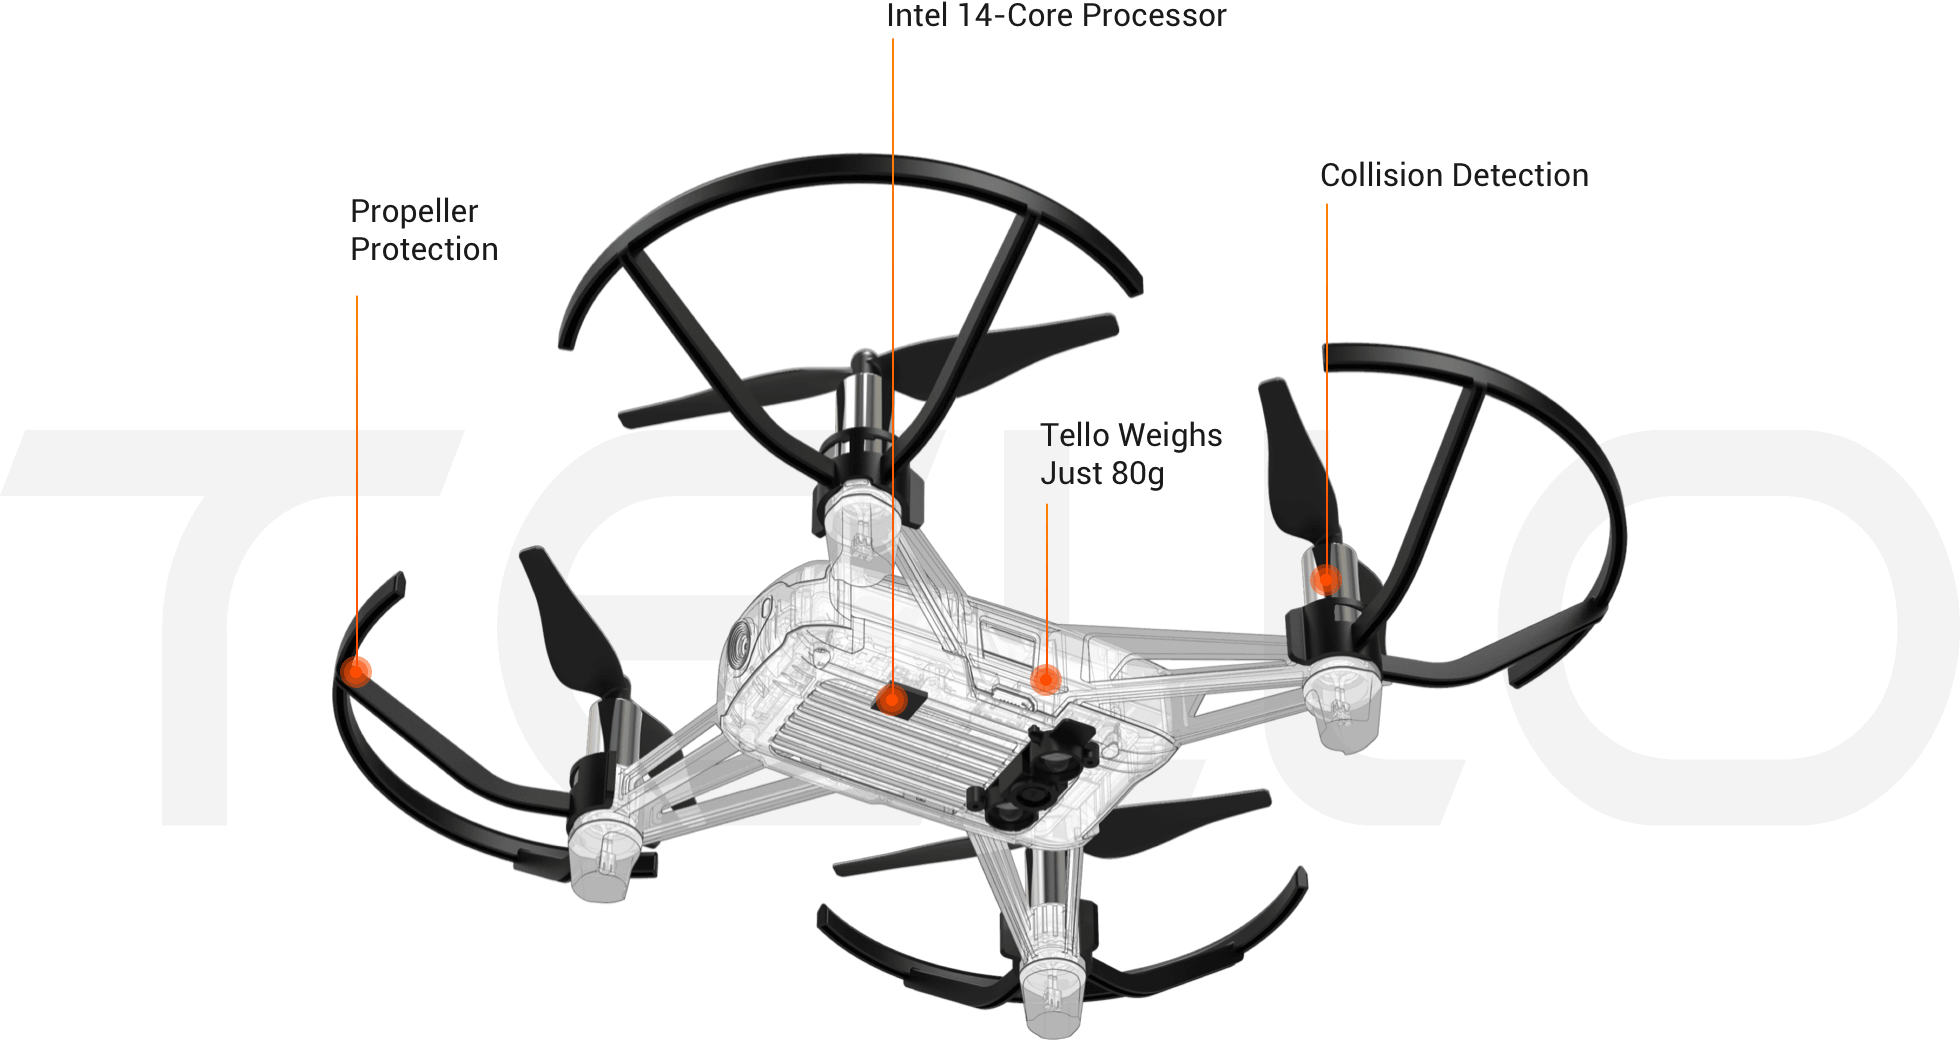
\includegraphics[width=0.75\linewidth]{img/tello}
	\label{fig:tello}
	\caption[Image of the Tello drone.]{Image of the DJI Tello drone. Source: \citep{tello}}
\end{figure}

\pagebreak
\section{Time Scope}
This project has been carried out over a period of 5 months, starting from September 2019 until January 2020. Within this period a couple of milestone dates exist, which were defined by \gls{FHTenL}. These dates can be found in the table below:
\begin{table}[h]
	\centering
	\begin{tabular}{|l|l|}
		\hline
		\textbf{Deliverable} & \textbf{Deadline} \\ \hline
		Project Plan & 27/09/2019 \\
		Midterm Report & 21/10/2019 \\
		Midterm Presentation & 11/11/2019 \\
		Thesis Report & 13/01/2020 \\
		Final Presentation & 27/01/2020 \\ \hline
	\end{tabular}
	\caption{List of school deadlines.}
	\label{tab:deadlines}
\end{table}

\section{Risk Analysis}
In order to minimize damage caused by risks, a risk analysis has been carried out. This has resulted in the creation of a risk matrix, which, due to its size, has been moved to appendix \ref{app:risks}. The matrix contains a list of risks, the consequences, and its scores based on the likelihood and impact. It also contains a mitigation plan to reduce its score, together with a set of new scores based on the effect of the mitigation.

\section{Project Justification}
\begin{table}[h]
	\centering
	\resizebox{\textwidth}{!}{%
		\begin{tabular}{l|l}
			\textbf{Description} & \textbf{Estimated values} \\ \hline
			Amount of locations & 80000 \\
			Times counted & 3 \\
			2nd and 3rd counts & 1000 \\ \hline
			Total locations ((amount of locations + 2nd and 3rd counts) * times counted) & 243000 \\
			Average time (seconds) per location & 30 \\ \hline
			Total work hours per annum & 2025 \\
			Amount of employees & 2 \\
			Warehouse employee cost per hour (euros) & 20 \\ \hline
			\textbf{Total costs warehouse employees (euros)} & 81000 \\
			\textbf{Total costs (including office employees and forklift costs) (euros)} & 95000
		\end{tabular}%
	}
	\caption[Estimated annual costs of cycle counts for 2020]{Estimated annual costs of cycle counts for 2020, based on a 30 second average per location.}
	\label{tab:costs}
\end{table}
One might wonder why instead of improving inventory control processes not improve picking and storing processes. While it is true that, in the absolute ideal case where storing and picking happens flawlessly, maintenance processes such as \gls{cycle_count}s wouldn't need frequent occurrences. However, considering that humans are involved in these processes it is safe to assume human mistakes will happen. Moreover, as warehouse employees are getting scarcer, the standard for hiring new employees keeps lowering, which results in more mistakes happening.
\\\\
According to \gls{CBS}, the working sector for transport and storage had roughly 8000 work-related injuries with a 4+ days absence occur in 2017. This ranks this sector the 4th highest sector with the most reported 4+ days absence work-related injuries, and the second-highest sector when looking at the percentage of employees sustaining injuries in comparison to the total number of employees in that sector \citep{cbs}.
\\\\
As seen in table \ref{tab:costs}, the estimated costs for 2020 is roughly \euro95000, of which \euro81000 goes to employees performing the cycle counts. Using drones could reduce the number of hours of those employees significantly, and thus reduce the largest cost in the whole cycle count process. It is important to note that the numbers used in this table have been altered slightly for privacy reasons.


	\chapter{Approaches}
\lhead{ \thechapter \space Approaches}
\label{ch:approaches}
This chapter covers the research done on potentially feasible \gls{AI}-based approaches.

\section{Multi-Objective Deep Q Networks with Subsumption Architecture}
Originally described by Rodney Brooks, it could be considered the opposition of \gls{AI}. This is due to the fact that subsumption architecture makes use of sensory input to layer competences, instead of being guided by mental/behavioral-based algorithms like \gls{AI} algorithms typically are \citep{subsumption_architecture}.
\\\\
A paper by Tomasz Tajmajer describes a solution that combines a multi-objective \gls{DQN} with signal suppression known from subsumption architecture to control a floor cleaning robot in a physical environment. As the paper explains, it makes use of separate \gls{DQN}s (A deep learned form of reinforcement learning) to determine the next action for each of the sub-tasks (floor cleaning, collision avoidance, recharging), which then get combined into one singular output that determines the next action. To create a single output, however, signal suppression is used to create a hierarchy among sub-tasks. For example, if the cleaning robot were to simultaneously have to avoid collision and recharge, it would most likely end up in it colliding as one task commands the robot the move and the other commands it to halt. To avoid this, the collision avoidance task is able to suppress the recharge task in order for the robot to prioritize its safety first \citep{mdqns}. This approach could be used for this project, where example sub-tasks could be collision avoidance and moving to a location.

\section{Object Detection-Based}
\label{sec:ssd_segmentation}
\gls{SSD} is a method that uses a convolutional neural network to detect objects in a single frame. Its detection speeds are very high, making it very suitable for real-time detection \citep{ssd}. An approach could be to train an \gls{SSD} to detect common objects that the drone needs to avoid. As the sizes of the objects are known roughly, a distance estimation can be made based on the pixel size. Alternatively, a \gls{RCNN} can be used. As the name suggests, it differs from a regular convolutional neural network in the way that it adds another layer to the Faster \gls{RCNN} model that creates a segmentation mask around the object in the bounding box, without the significant loss of performance (real-time speed of 5 frames per second) \citep{mask_cnn}. Just like the Faster-\gls{RCNN} it is based on, it makes use of Region Proposal Network that creates rectangles around potential objects and scores them based on their membership to object classes vs. the background \citep{faster_rcnn}. A project by Waleed Abdulla presents an implementation of a Mask \gls{RCNN} \citep{matterport}, which could then be used to estimate the distance with. While the distance estimation would be more accurate with the latter approach, it comes at the price of a drop in processing speed and thus frame rate.

\section{Unity Machine Learning Agents}
\label{sec:approach_ml_agents}
\gls{unity} is an open-source game engine used for creating 2D and 3D games/simulations. In 2017, Unity introduced a toolkit called \gls{mlagents}, which enables users to use reinforcement learning on their Unity environments \citep{mlagents_blog, mlagents_paper}. The approach would then be to create a somewhat realistic simulation of a warehouse to train an algorithm on, and then later use the trained algorithm on a real drone. An example of this would be the solution presented by Adam Kelly, who created a simulation for training airplanes to fly through waypoints \citep{ai_flight}.
\\\\
An alternative approach could be to make use of imitation learning instead of regular reinforcement learning to train the algorithm. At a Unity event called Unite, Unity gave a number of demonstrations of \gls{mlagents} applications. Among these demonstrations was a racing game, where the algorithm learned to copy the human player's behavior through imitation learning \citep{imitation_learning, mlagents_paper}. This could be used to learn the drone to autonomously fly to certain points in the warehouse while avoiding collisions.

	\chapter{Concept 1: Unity Machine Learning Agents}
\lhead{\thechapter \space Concept 1: Unity Machine Learning Agents}
\label{ch:concept_one}
The first concept chosen was the \gls{mlagents} approach mentioned in section \ref{sec:approach_ml_agents}. This chapter describes the concept of this approach, the reasons for choosing this approach over the others, the simulation built, and the results.

\section{Concept Description}
As the drone only comes with a monocular, front-facing camera to sense its environment with, either the use of traditional computer vision-based or an \gls{AI}-based algorithm (or a combination) seemed like the most straightforward options. A high-paced and somewhat chaotic environment such as a warehouse seemed like an interesting case for \gls{AI}. Seacon was particularly interested in this solution as an \gls{AI} solution might have had the ability to simultaneously and seamlessly handle multiple tasks at once. This resulted in the creation of a concept where drones would start from a base station located somewhere in the warehouse, and would fly to desired locations while avoiding collisions with objects. Since the scope is limited to a single warehouse layout, and warehouses often having random objects/people at unpredictable locations, the simple use of a map was not considered a robust solution. Thus, an \gls{RL} solution was opted for.

\section{Preliminary Research for Simulation}
As drones are relatively expensive, have a limited battery life, and have a risk of getting damaged it was decided to develop a simulation. As the most-widely used language for \gls{RL} is Python, it was decided to also have a Python-native simulation environment. This would ease exchanging values between the simulation and the \gls{RL} agent. Multiple existing drone flight simulators were created and published by Simon Levy \citep{simon_github}. Out of these projects the PyQuadSim (see figure \ref{fig:pyquadsim}) project seemed most suitable, as it was based on Python and lightweight. However, in the end it was decided that to create an own simulation as it requires for it to be as realistic as possible to the real world application \citep{mit_rl}. To shorten development times needed, the \gls{unity} engine was chosen.
\begin{figure}[h]
	\centering
	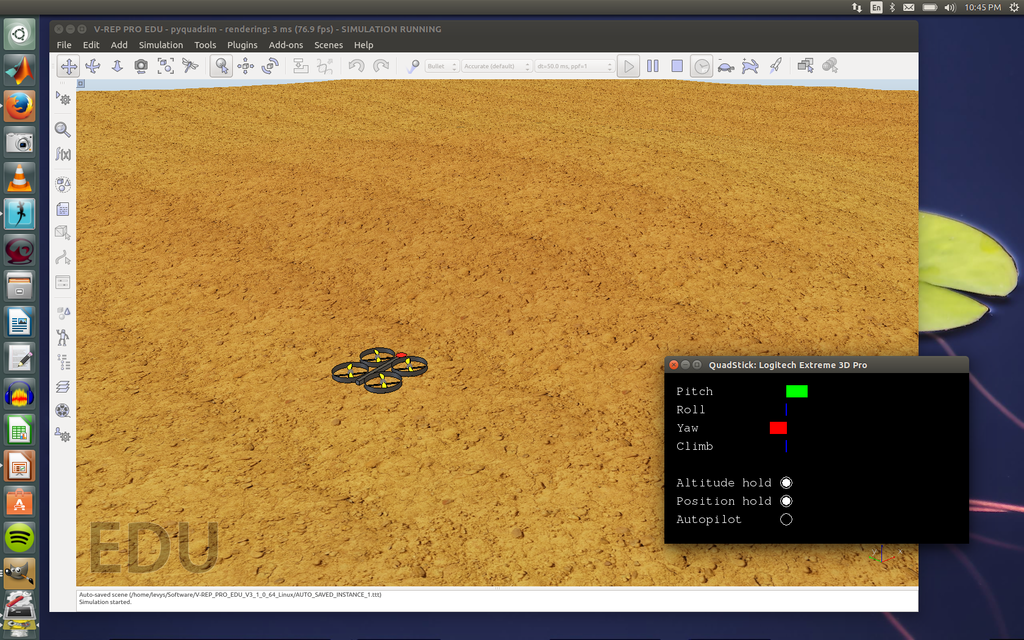
\includegraphics[width=0.75\linewidth]{img/pyquadsim}
	\label{fig:pyquadsim}
	\caption[Screenshot of the PyQuadSim project]{Screenshot of the PyQuadSim project. Source: \citep{pyquadsim}}.
\end{figure}
\pagebreak

\gls{unity} was chosen over alternatives for 2 reasons. Firstly, the company had experience with developing products using this engine. This opened up the opportunity for the company to do code reviews and generally being able to provide tips. Moreover, a realistic model for the drone and a variety of warehouse assets were available. The second and most important reason for choosing Unity, however, was \gls{mlagents}.

\section{Unity Simulation}
The original simulation can be seen in figure \ref{fig:first_sim}. It was made so each time the warehouse was generated, it would have a random size and amount of racks ranging from 1 to 8 racks. It was also equipped with an option to turn on or turn off training mode. Turning on training mode would minimize graphical load by replacing the models with simpler shapes and textures, as seen in the right image of figure \ref{fig:first_sim}.

\begin{figure}[h]
	\centering
	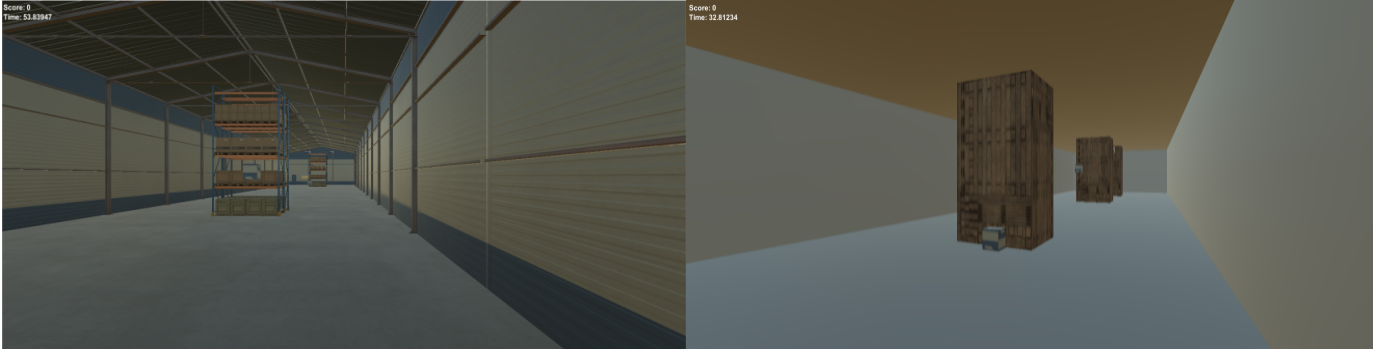
\includegraphics[width=\linewidth]{img/unity_real_training}
	\label{fig:first_sim}
	\caption{First design of the Unity warehouse simulation.}
\end{figure}

Based on feedback by the company the design was changed to feature 2 long rows of racks instead, as this was considered closer to the real situation. This was changed as displayed in figure \ref{fig:second_sim}, while maintaining the option for toggling training mode and a variable warehouse length. Both designs also featured targets spawning in at random positions in front of the racks. These targets functioned as an indication for where the drone should fly, and would grant the drone an increase in score whenever the drone flew over it. The simulation was made so that the view on screen simulated the view a real drone would have through its front-facing camera.

\begin{figure}[h]
	\centering
	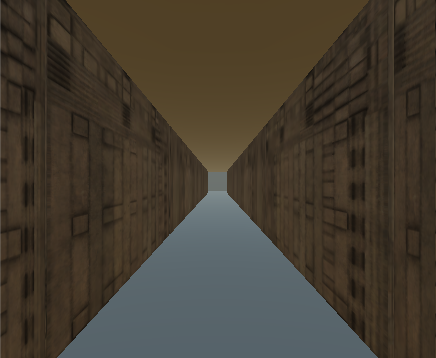
\includegraphics[width=0.5\linewidth]{img/sim_reinforcement}
	\label{fig:second_sim}
	\caption{Updated design of the simulation in training mode.}
\end{figure}

\section{ML-Agents Classes }
The implementation of the simulation with \gls{mlagents} contains 4 major parts: generator classes, the Unity package, the \gls{mlagents} package and its inheriting classes, and the class for reading a configuration file. Since the Unity package is the default package that all c\# Unity projects use, it will not be discussed here. A class diagram can be found in appendix \ref{app:sim_class_diagram}.

\paragraph{Generator} Generator is an abstract class that has concrete implementations for spawning the drone, warehouse, and the targets. Using the strategy design pattern, all the generators are registered and invoked by the DroneAcademy class.

\paragraph{DroneAcademy} DroneAcademy inherits from the Academy class within the ML-Agents package. It is responsible for all operations around the environment during training, for example destroying or adding new objects to the scene.

\paragraph{DroneAgent} DroneAgent inherits from the Agent class within the ML-Agents package. The object containing an implementation of the Agent class is meant to be controlled by a neural network (or "brain" in the context of Unity) during training.

\paragraph{ConfigHandler} ConfigHandler reads an external configuration file that contains information about how to generate the scene. Examples include the size of the warehouse and whether or not to enable training mode.

\section{Reinforcement Learning \& Imitation Learning}
For the \gls{RL} implementation the standard models provided by \gls{mlagents} were used. The \gls{RL} implementation was given the drone's coordinates, horizontal and vertical velocity, camera input, as well as the target's coordinates as input. The drone (or "agent" in \gls{RL} lingo) then was given 10-60 seconds (based on the warehouse size) to reach its target, and was rewarded based on its time left after reaching its goal. The agent was also mildly penalized for moving, in order to motivate it to keep its movement to a minimum. Once the agent had reached its target, the environment would reset and the warehouse would be regenerated using a random size, and the end of a so-called episode would then be reached. The ending of an episode means that the total reward score for that lifetime is finalized. In case the drone would crash into something, the episode would end immediately and the total reward score would be the lowest possible. Unfortunately, after having run several training sessions spanning somewhere between 10 minutes and 3 hours, the agent did not seem to learn. It kept flying a similar pattern, where it would fly up and slightly left or right, crashing into the ceiling. 
\\\\
As alternative, another model provided by \gls{mlagents} was used. This model, however, was for \gls{IL}. While they are both genetic algorithms, the major difference between \gls{IL} and \gls{RL} is that \gls{IL} does not make use of a predefined reward function. Instead, it tries to derive that function by imitating an expert (human) player. As a result, the simulation was slightly altered to spawn 2 identical warehouses that allowed for multiplayer (human vs. agent), as seen in figure \ref{fig:sim_imitation_scene_training}. To monitor progress, the simulation was altered to display both the view of the human-controlled drone and the agent-controlled drone in a split screen manner. This, however, also did not show any significant results. Even after having provided demonstrations for an hour, the agent kept moving slowly until it crashed in its nearest object, and did thus not show any sign of learning.
\begin{figure}[h]
	\centering
	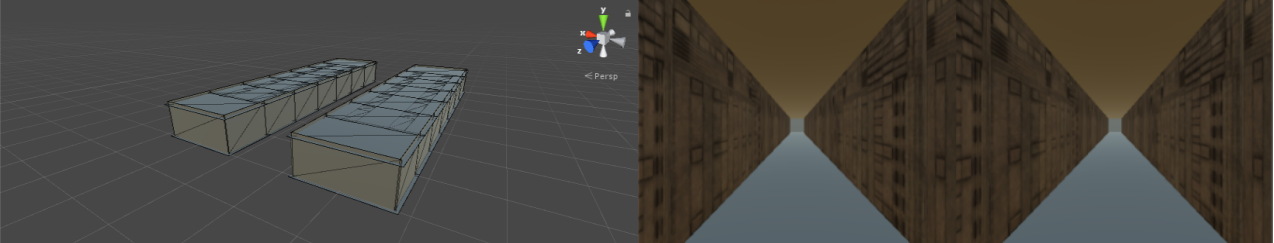
\includegraphics[width=\linewidth]{img/sim_imitation_scene_training}
	\label{fig:sim_imitation_scene_training}
	\caption[Simulation altered for running for imitation learning]{Simulation altered for running for imitation learning. The left image shows the warehouses from the outside, and the right image shows the view seen during training.}
\end{figure}


	\chapter{Concept 2: State Machine Implementation}
\lhead{\thechapter \space Concept 2: State Machine Implementation}
\label{ch:concept_two}
Based on feedback received during the midterm presentation, it became clear that drastic changes needed to happen, mainly due to an improper requirements analysis. Since the concept described in chapter \ref{ch:concept_one} did not show promising results, it was decided to switch to a new concept in order to reduce the risk of not having a (partially) working product at the end. Through a brainstorm session with the company a new concept was developed. In order to combat time constraints, it was decided to limit the scope to just one side of a rack, instead of covering the whole warehouse. Further details regarding this concept are explained in the remainder of this chapter. Installation instructions and a guide for running the project can be found in appendix \ref{app:setup}.

\section{Product Functions}
\label{sec:product_description}
The goal of this project is mainly focused on developing a solution for providing a drone with collision avoidance. However, along the course of the project it became evidently clear that a indoor self-flying (figure \ref{fig:roadmap}) component was also necessary. From here on out, the functions could be divided among the 3 dimensions the drone has to interact with as follows:
\begin{figure}[h]
	\centering
	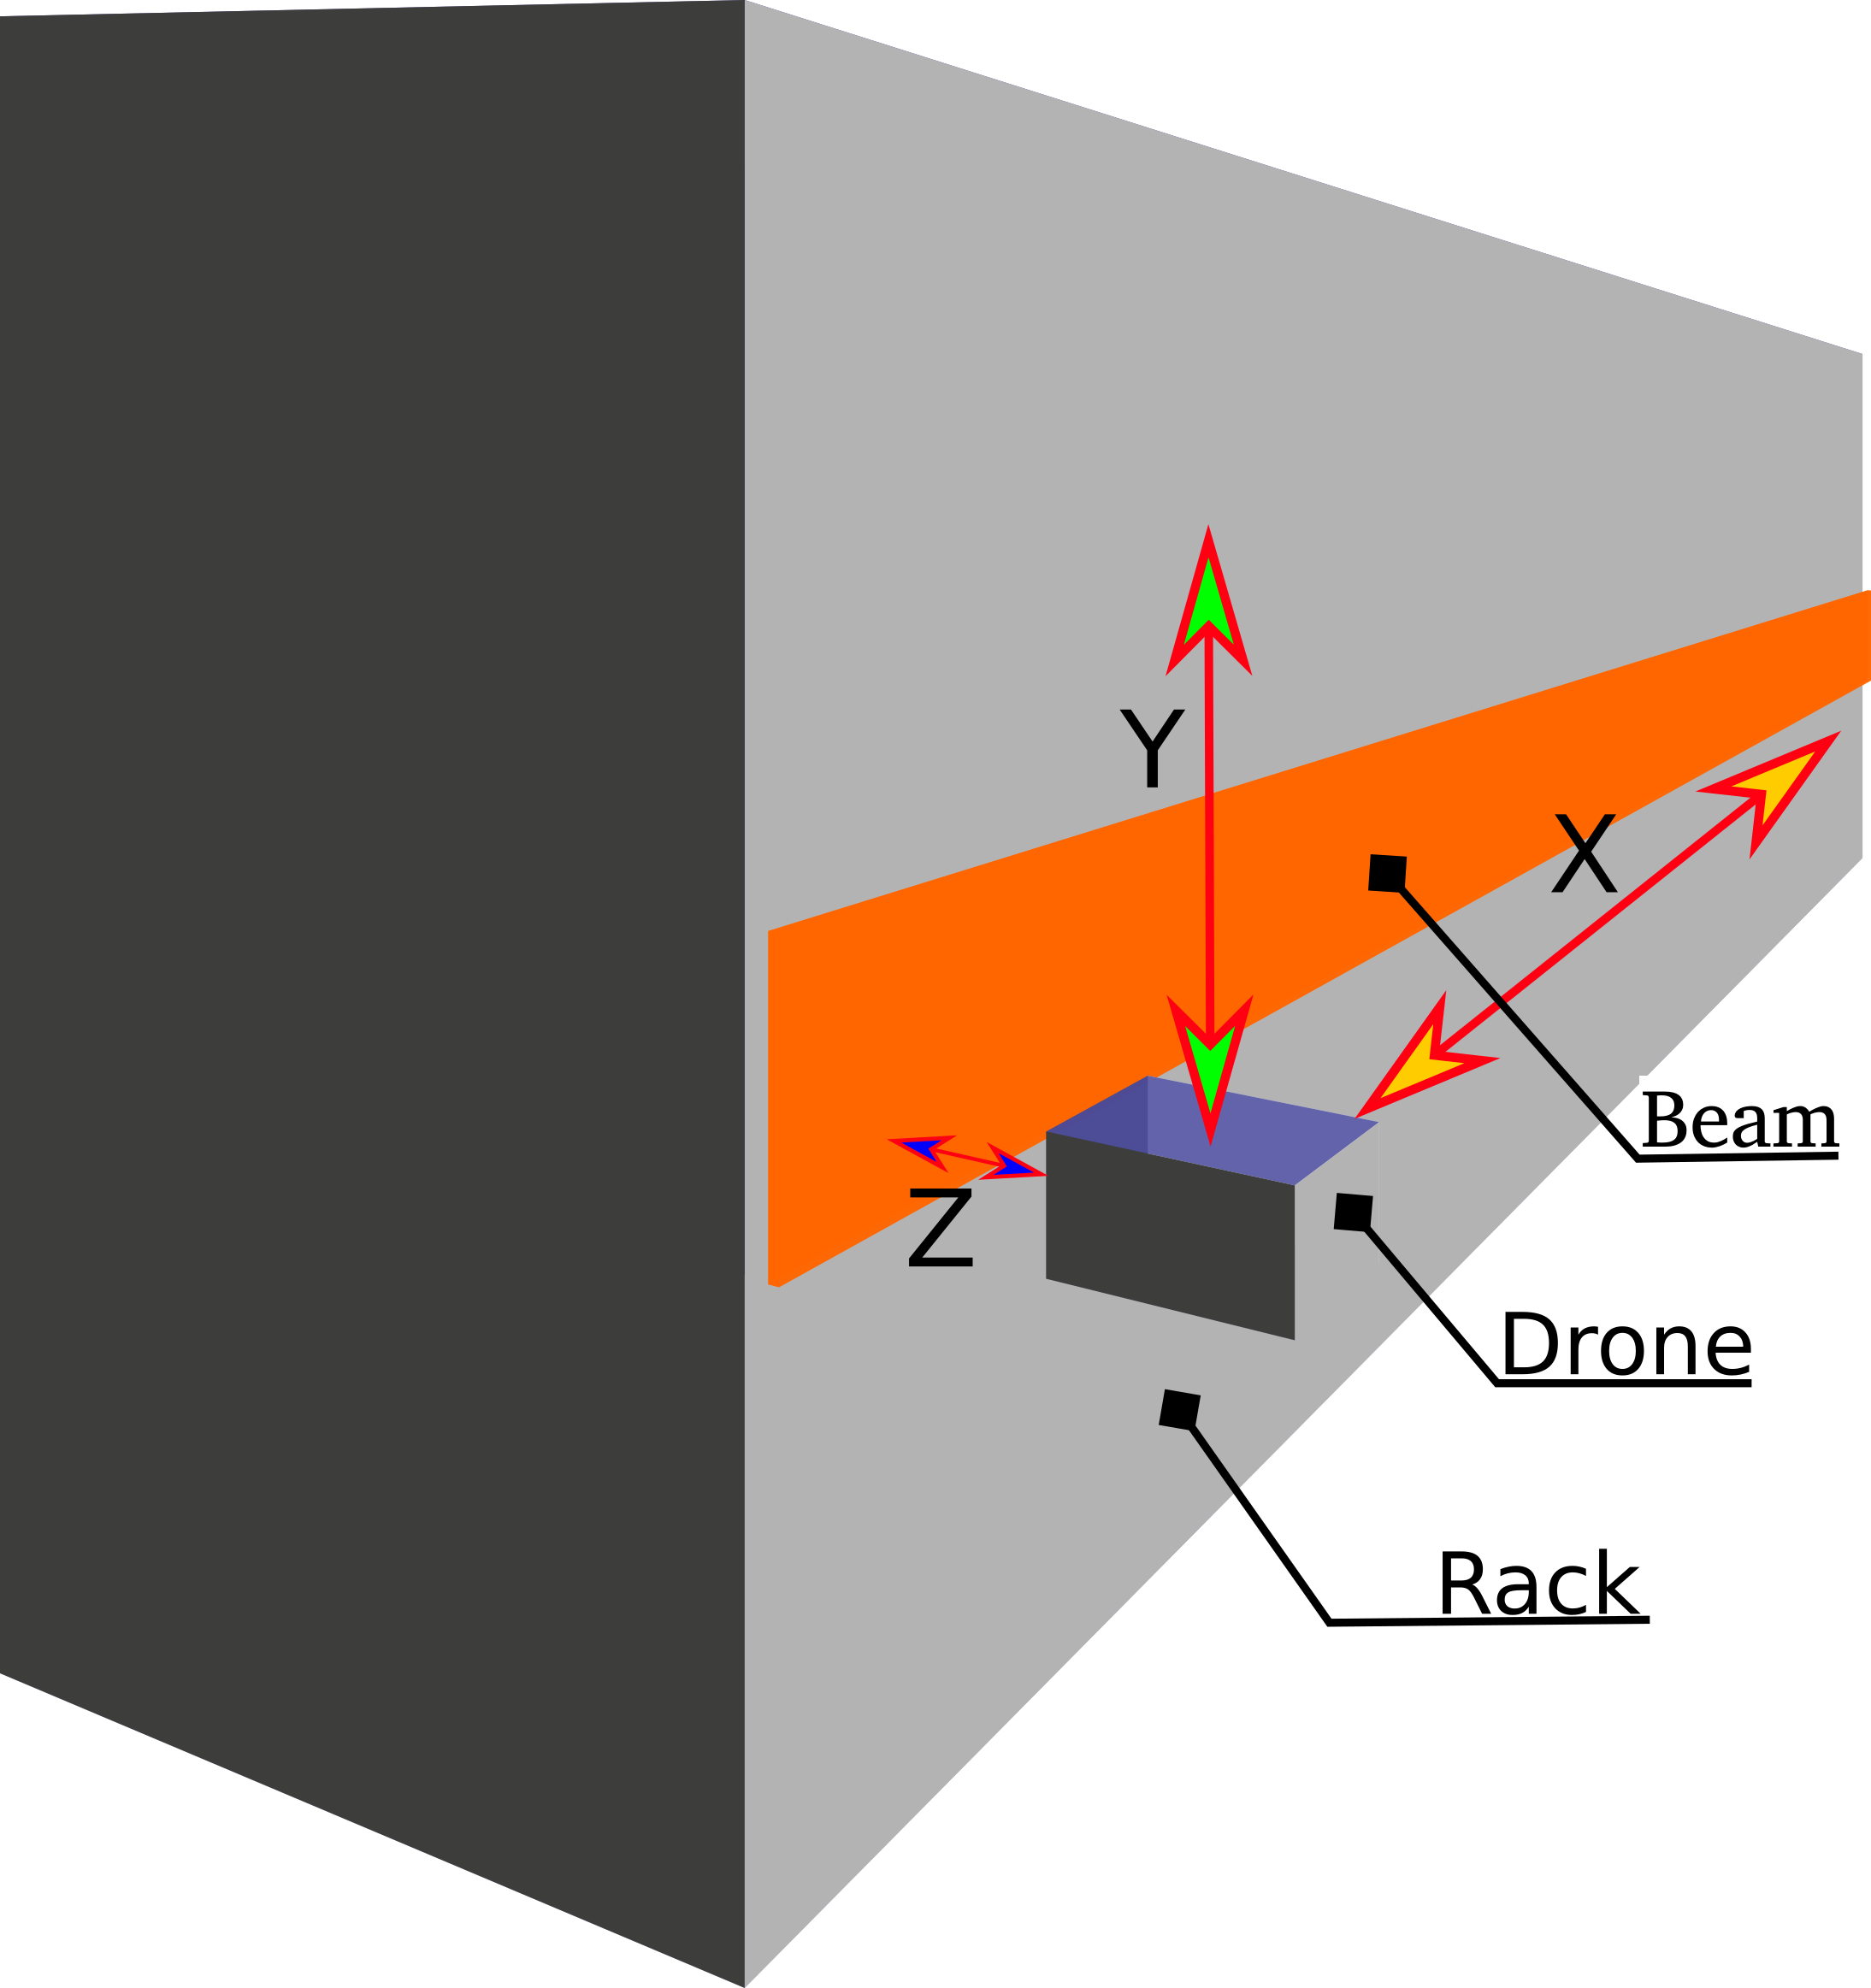
\includegraphics[width=\linewidth/2]{img/drone_concept_diagram}
	\label{fig:drone_concept}
	\caption{Visual representation of the single rack concept.}
\end{figure}

\begin{itemize}
	\item X-axis:
	\begin{itemize}
		\itemsep0em
		\item Move the drone sideways
		\item Stop the drone at the end of a bar
		\item Detect objects in the drone's trajectory
		\item Avoid collisions with objects in the drone's trajectory
	\end{itemize}
	\item Y-axis:
	\begin{itemize}
		\itemsep0em
		\item Keep the bar in the center of the drone's camera
		\item Change the drone's altitude to switch layers
		\item Keep track of the current layer and the highest layer
	\end{itemize}
	\item Z-axis:
	\begin{itemize}
		\itemsep0em
		\item Estimate the pixel size of the bar
		\item Keep the drone to maintain distance from the bar
	\end{itemize}
\end{itemize}
This list is originally taken from the \gls{SRS} in appendix \ref{app:srs}. Figure \ref{fig:drone_concept} contains a visual representation of the concept with its functions.

\section{State Machine}
The initial state design featured a concept where the drone correct its positions for safety, move sideways viewing the beam at set intervals and then do a check for objects in its trajectory. This design is displayed in appendix \ref{app:bar_states_simple}. However, it was decided to shift to a design that selects a state based on a set of criteria (see table \ref{tab:criteria}) so that states such as checking for collision or locking-on can happen more frequently. For the second state machine design, please refer to appendix \ref{app:bar_states_two}. It is important to note that as of writing this document, the states "moving layer" and "returning home" have not been implemented yet due to time constraints. The state "avoiding collision" has only been partially implemented, where it only determines if an object is too close and then proceeds to land accordingly. Descriptions of all implemented states can be found in table \ref{tab:state_desc}.
\begin{table}[h]
	\centering
	\resizebox{\textwidth}{!}{%
		\begin{tabular}{lll|l}
			\textbf{} &  &  & \textbf{Transition to state:} \\
			\textbf{Criteria:} & Locked on? & Distance interval reached? & \cellcolor[HTML]{9B9B9B}{\color[HTML]{333333} } \\ \hline
			& False & False & Locking on \\
			& False & True & Locking on \\
			& True & False & Advancing \\
			& True & True & {\color[HTML]{333333} Rotating to hall}
		\end{tabular}%
	}
	\caption{Table displaying state transitions from the facing bar state, based on 2 criteria.}
	\label{tab:criteria}
\end{table}

For simplification, the currently implemented state machine can be grouped into 3 group states: locking on, checking for collision, and advancing. Here, locking on refers to centering the beam in its view and maintaining an appropriate distance, checking for collision refers to rotating the drone to check the hallway for objects in its trajectory, and advancing refers to moving the drone sideways along the beam. The criteria "Locked on?" is currently set to false after having completed any of the aforementioned group states (aside from "locking on", which sets it to true again). "Distance interval reached?" is set to true after exiting the advancing group state, and back to false after exiting "checking for collision".

\begin{table}[h]
	\centering
	\resizebox{\textwidth}{!}{%
		\begin{tabular}{l|l}
			\textbf{State} & \textbf{Description} \\ \hline
			Facing beam & The drone is hovering in front of the beam while facing it. Also acts as a central state. \\
			Locking on & The drone is positioning itself to center the beam and maintain its distance from it. \\
			Advancing & The drone is moving sideways along the beam. \\
			Rotating hall & The drone is rotating towards to hall to prepare to check for collisions. \\
			Detecting collision & The drone is using background subtraction to check for objects in its near trajectory. \\
			Avoiding collision & The drone determines if an object is too close and lands to avoid collision if necessary. \\
			Rotating beam & The drone rotates back so it is once again facing the beam.
		\end{tabular}%
	}
	\caption{Implemented states with descriptions of what happens during their executions.}
	\label{tab:state_desc}
\end{table}

\section{Implementation}
\label{sec:implementation_two}
The implementation is written in Python and makes use of 3 main components: OpenCV, transitions, and the Tello-openpose project. OpenCV is a computer vision library \citep{opencv}, transitions is a Python package that provides state machine implementation functionality \citep{transitions}, and Tello-openpose is a project by Github user Geaxgx that enables a Tello drone to track a human and follow commands via gestures \citep{tello_openpose}. The last component mentioned was used as the basis for this project, but has since been modified significantly.
\\\\
The product contains the following scripts with the following responsibilities:

\paragraph{Main.py:} Used to run the product, primarily responsible for invoking the other scripts, connecting to the drone, and running a loop to obtain the frames.

\paragraph{DroneController.py:} Communication script between the other scripts and the drone. It stores information about the drone, handles the logs, and provides functionality for controlling the drone either through functions or by keyboard. This script was based on the Tello-openpose project, and makes use of a Python package called Tellopy that provides a set of functions for the scripted controlling of a Tello drone \citep{tellopy}.

\paragraph{BeamDetector.py:} Provides functions that get an estimate of the edges of a beam. This happens by using OpenCV to get a binary (either black or white pixels) image, get the contours, and then obtain all straight lines from the contours using a function called \gls{houghLinesP}. To filter out noise, the script also gets the average Y-coordinate of all lines to create a pivot, and then groups them together into a lower-half and upper-half group. The respective averages of those 2 groups then form the upper-edge and lower-edge of the beam.

\paragraph{DistanceEstimator.py:} Provides functions for getting the distance between the center of the beam and the camera center, as well as a function for estimating the distance based on the size of the beam in pixels. The former is done by providing the frame width, frame height, and the minimal and maximal Y-coordinate found using the functions of BeamDetector.py.

\paragraph{CollisionDetector.py:} Provides functions that can distinguish foreground objects from background objects, get the contour size from the foreground objects and use that to very roughly estimate the proximity based on the amount of space the contour takes up in the frame. For reference, please look at figure \ref{fig:collision_detection}. The top two images are frames directly from the drone camera, and the bottom two are the same frames where background subtraction has been applied. In the images of the left column the drone is at a safe distance, while in the right column it is too close, hence why the bottom right image has a "Danger" tag in it.

\paragraph{StateMachine.py:} Makes use of the transitions Python package to define the states, the possible state transitions, and the conditions for transitioning. Also stores a time stamp of the time when the most recent state enter has occurred.
\begin{figure}[h]
	\centering
	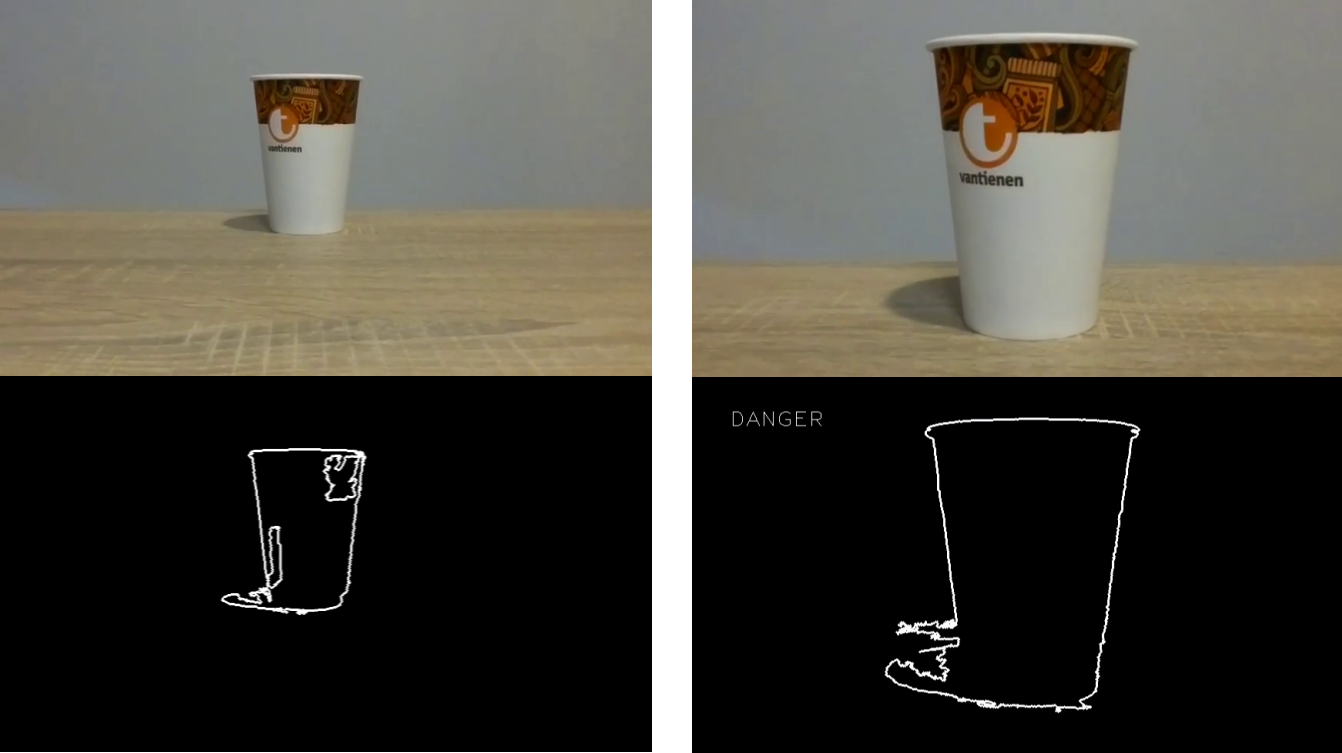
\includegraphics[width=\linewidth]{img/collision_detection_sample}
	\label{fig:collision_detection}
	\caption{Set of images demonstrating collision detection.}
\end{figure}

\paragraph{StateMachineActions.py:} Acts as a bridge between StateMachine.py and DroneController.py. It has an execute function that checks the state of the StateMachine instance and invokes a function accordingly. It also checks when a state can be exited, and updates the criteria seen in table \ref{tab:criteria}. For example, when the StateMachine instance has entered the "advancing" state, StateMachineActions will invoke the function in DroneController that will make the drone move sideways until the interval is reached. Then it will update the criteria and use the transition to go back to the "facing bar" state.

\paragraph{FPS.py \& HUD.py:} As Main.py displays the camera frames in a window, HUD.py adds and updates textual information to each frame. FPS.py calculates the frames per second, which is in turn used by HUD.py. The code of both these scripts originated from the Tello-openpose project.
\pagebreak
\section{Limitations \& Problems}
\label{sec:state_machine_limits}
The current product faces 2 major issues. The biggest issue is the limitations of classical computer vision algorithms, on which the product is highly dependent on. A lot of averaging has been done in an attempt to minimize noise, however it seems that the distance and lighting range in which the product operates normally is still rather small. Another major issue is the communication with the current drone. It only accepts one command at a time sent by an UDP-protocol ("single shot" message-oriented communication protocol), which might cause the software and the drone to desynchronize. To clarify, listing \ref{lst:error_log} displays the debug log while running the Main.py script. Each 0.2 seconds the current state is printed. However, while in line 2 and 3 it shows the command is received by the drone fairly quickly after switching states (at least within 0.2 seconds), it does not to seem to be the case when rotating back at lines 6-8. This causes the drone to not rotate back all the way (due to the duration of the rotation being an estimate based on speed and distance) and ultimately causes it to stop functioning properly.
\begin{lstlisting}[caption={Fragment excerpted from the debug log of the product.},captionpos=b,label={lst:error_log}]
facing bar
Rotating to hall
Tello: 14:44:45.588:  Info: clockwise(val=100)
...
Avoiding collision
Rotating to bar
Rotating to bar
Tello: 14:44:48.224:  Info: clockwise(val=-100)
Rotating to bar
Stopping rotation
Tello: 14:44:48.494:  Info: clockwise(val=0)
facing bar
\end{lstlisting}

One minor improvement point is that the distance between the camera center and the center of the beam is still measured in pixels, while the distance between the drone and the beam is in metric units. For consistency purposes, this should be changed to the same format.
\\\\
There are also a couple of limitations caused by the Tello drone. To be able to stabilize itself, it makes use of an infrared camera that points to the surface it is hovering over. However, the requirements for this to work are rather strict. It seems to respond badly to uneven surfaces (think of flying over small objects such as doorsteps), reflective surfaces, and dark or monochrome surfaces. The issue with this is that, especially in the case of uneven surfaces, the drone will force itself to correct its position, and thus overrule any other input. This might cause issues when a drone were to fly over a box on the ground at a low altitude as the script receives very little information about the drone's status, causing it to ultimately desynchronize. Another limitation is its battery life, which, after testing, spans roughly 10 minutes.

%TODO:add class diagram?
%TODO: Elaborate on computer vision pipeline
	\chapter{Conclusion}
\lhead{\thechapter \space Conclusion}
\label{ch:conclusion}
The Warehouse Drone Collision Avoidance project resulted in the development of 2 concepts: an \gls{AI}-based one using Unity's ML-Agents and a state machine implementation one. This chapter gives a short summary of each of the concepts and draws a conclusion.

\section{Machine Learning Agents \& Research}
For the \gls{mlagents} concept a Unity environment was developed that could simulate a warehouse with variations. Using the \gls{mlagents} toolkit several training sessions were run. This concept, however, did not show any signs of learning after having trained it for 3 hours for \gls{RL} and 1 hour for \gls{IL}. After having done more research, it can be concluded that reinforcement learning as stand-alone solution will not suffice. This is due to the fact that rewards are very sparsely distributed, which is generally handled badly by \gls{RL} algorithms. Moreover, as environments get increasingly complex, the risk of the algorithm getting stuck in local optima or finding an out-of-the-box answer that gives a better reward than the intended answer increases \citep{rlblogpost}. An example is the paper by \gls{AI} research company OpenAI on a game where 4 agents are tasked to play hide and seek in teams of 2. In the paper, it is described that eventually the agents started finding several exploits in the physics engine of the game, with an example being abusing the contact physics to force a ramp to go through the wall separating the play area \citep{hideandseek}.
\\\\
Based on the results and the risk of not having selected a viable approach, it was decided to switch to the state machine concept after the midterm presentation. This was done as a (partially) working product was favored over continuing the research.

\section{State Machine Concept}
Unlike the \gls{mlagents} approach, the state machine concept limited its scope to just one side of a rack. Through the use of a state machine, the product is able to switch tasks based on a set of criteria. Currently included tasks are: finding the vertical distance between the center of the camera and the center of the beam, estimating the distance between the drone and the beam, moving sideways, rotate, distinguish the foreground from the background, and make a rough estimation of how close an object is. Although the product contains an implementation for all these tasks, it is concluded that it is not ready for a practical environment yet. Tests using the Tello drone show that the product still has insufficient control over the drone, and is still too susceptible to noise. Furthermore, the drone still contains some bugs and improvement points, such as the rotation bug mentioned in section \ref{sec:state_machine_limits} and the fact that the collision detector its performance is based on well the drone can maintain its position. With some optimization, however,  it is believed that this concept could end up being usable in a practical environment such as a warehouse.

	\chapter{Recommendations}
\lhead{\thechapter \space Recommendations}
\label{ch:recommendations}
There are many ways to proceed with this project. This chapter describes the recommended ways to proceed, based on the work and research done. The recommendations listed focus on the improvement of the existing implementation, rather than extending it. 

\section{Computer Vision Enhancements}
The state machine concept is mostly reliant on its accuracy of its computer vision tasks. Enhancing these should result in a drastic increase in stability. There are, however, many ways to go about this. Currently, all computer vision tasks make use of a single frame. Adjusting this to make use of an average of a small number of frames should help out filtering noise without a significant loss in performance speed.

\section{Movement Enhancement with PID controllers}
One specific improvement possible is the improvement of the beam centering and distance maintenance (locking on state) task through the implementation of \gls{PID} controllers. \gls{PID} controllers makes use of a feedback loop control mechanism to regulate values. Using the beam centering as example, a \gls{PID} controller would make use of the present difference between center points (Proportional), how far it has already moved in previous iterations of the loop (Integral), as well as an estimate of how far it will end up afterwards (Derivative) for determining how much it should move the drone up or down. Proper use of this should result in not only in increase in positioning accuracy, but also an increase in performance speed.
\\\\
The Tello-openpose project that this product was based on made use of such controllers for tracking a human \citep{tello_openpose}. Due to difficulties with tuning them and time constraints, however, it was decided to leave them out at the time.

\section{Object Segmentation}
Continuing the research, the computer vision part can also be enhanced using the object detection/segmentation approach described in section \ref{sec:ssd_segmentation}. Using deep learned mask segmentation on the beam could provide a more accurate and robust solution to the distance estimation and beam centering tasks. It could also be used for collision detection, similarly to how the current implementation works. The model could be trained on common objects it has to mask. A distance estimation can then be made using its known average size together with the size of the mask. 
	
	%Bibliography
	\bibliographystyle{agsm}
	\bibliography{utility/bibliography}
	\lhead{\thechapter \space References}
	
	%Appendices
	\begin{appendices}
		\chapter{Drone States}
\lhead{\thechapter \space Drone States}
\label{app:drone_states}

\begin{figure}[h]
	\centering
	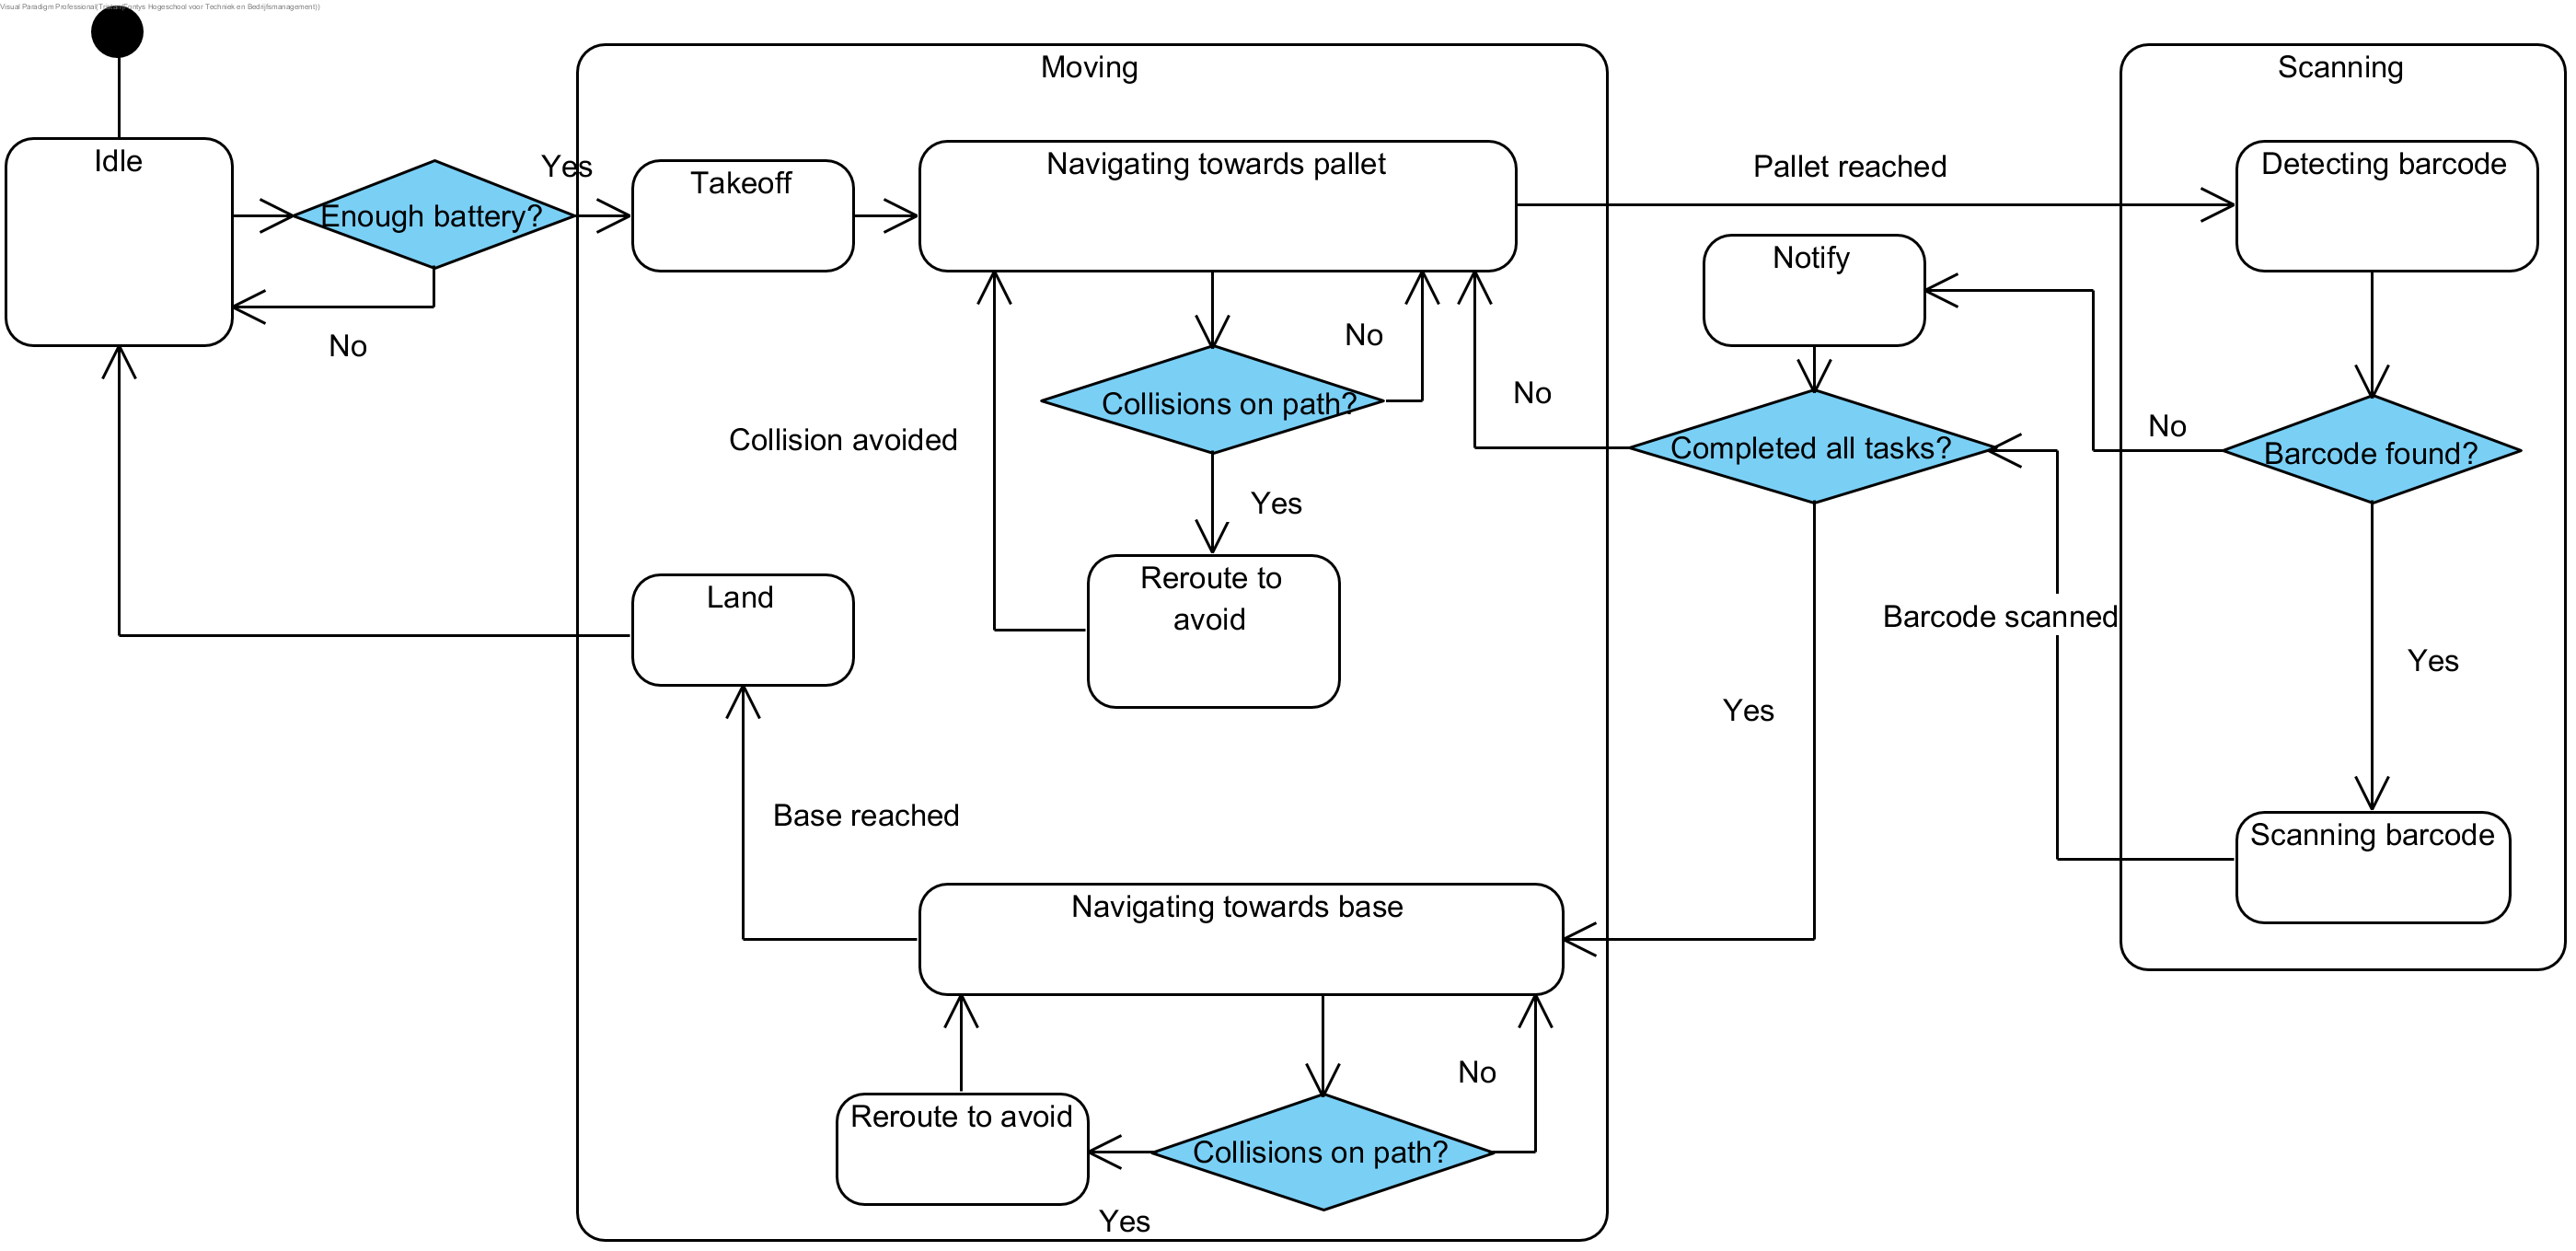
\includegraphics[width=\textwidth, angle=-90]{img/drone_states.png}
	\caption{State model of a drone performing inventory control}
	\label{fig:drone_states}
\end{figure}
		\chapter{Risk Management}
\lhead{\thechapter \space Risk Management}
\label{app:risks}

\begin{figure}[h]
	\centering
	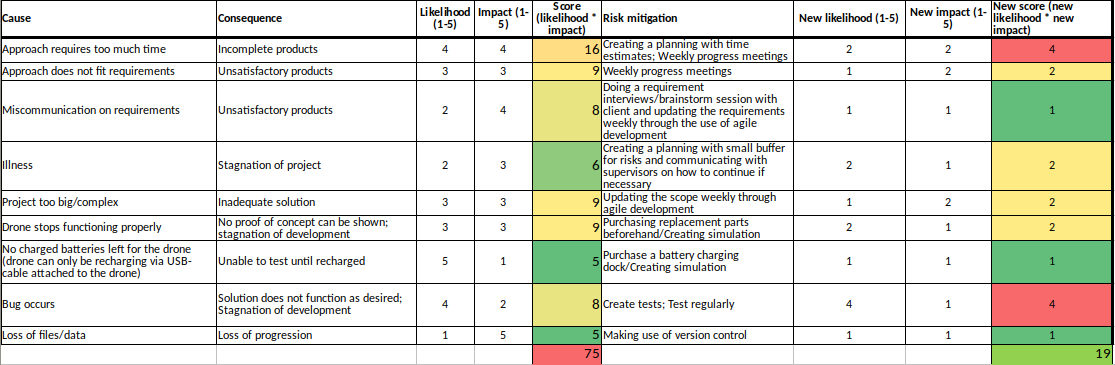
\includegraphics[width=\linewidth, angle=-90]{img/risk_matrix_post_midterm}
	\label{fig:risk_matrix}
	\caption{Risk matrix containing the risks with their mitigation plans.}
\end{figure}

% Please add the following required packages to your document preamble:
% \usepackage{graphicx}
%\begin{table}[]
	%\centering
	%\resizebox{\textwidth}{!}{%
		%\begin{tabular}{l|l|l|l|l|l|l|l|l}
			%\textbf{Cause} & \textbf{Consequence} & \textbf{Likelihood (1-5)} & \textbf{Impact (1-5)} & \textbf{Score (likelihood * impact)} & \textbf{Mitigation plan} & \textbf{New likelihood} & \textbf{New impact} & \textbf{New score} \\ \hline
			%Approach requires too much time & Incomplete products & 4 & 4 & 16 & Creating a planning with time estimates; Weekly progress meetings & 2 & 2 & 4 \\ \hline
			%Approach does not fit requirements & Unsatisfactory products & 3 & 3 & 9 & Weekly progress meetings & 1 & 2 & 2 \\ \hline
			%Miscommunication on requirements & Unsatisfactory products & 2 & 4 & 8 & Doing a requirement interviews/brainstorm session with client and updating the requirements weekly through the use of agile development & 1 & 1 & 1 \\ \hline
			%Illness & Stagnation of project & 2 & 3 & 6 & Creating a planning with small buffer for risks and communicating with supervisors on how to continue if necessary & 2 & 1 & 2 \\ \hline
			%Project too big/complex & Inadequate solution & 3 & 3 & 9 & Updating the scope weekly through agile development & 1 & 2 & 2 \\ \hline
			%Drone stops functioning properly & No proof of concept can be shown; stagnation of development & 3 & 3 & 9 & Purchasing replacement parts beforehand/Creating simulation & 2 & 1 & 2 \\ \hline
			%No charged batteries left for the drone (drone can only be recharging via USB-cable attached to the drone) & Unable to test until recharged & 5 & 1 & 5 & Purchase a battery charging dock/Creating simulation & 1 & 1 & 1 \\ \hline
			%Bug occurs & Solution does not function as desired; Stagnation of development & 4 & 2 & 8 & Create tests; Test regularly & 4 & 1 & 4 \\ \hline
			%Loss of files/data & Loss of progression & 1 & 5 & 5 & Making use of version control & 1 & 1 & 1 \\ \hline
			%&  &  &  & TOTAL = 75 &  &  &  & TOTAL = 19
		%\end{tabular}%
	%}
	%\caption{Risk matrix containing the risks with their consequences, scores, mitigation plans, and mitigated scores.}
	%\label{tab:risk_matrix}
%\end{table}
		\chapter{Simulation Class Diagram}
\lhead{\thechapter \space Simulation Class Diagram}
\label{app:sim_class_diagram}

\begin{figure}[h]
	\centering
	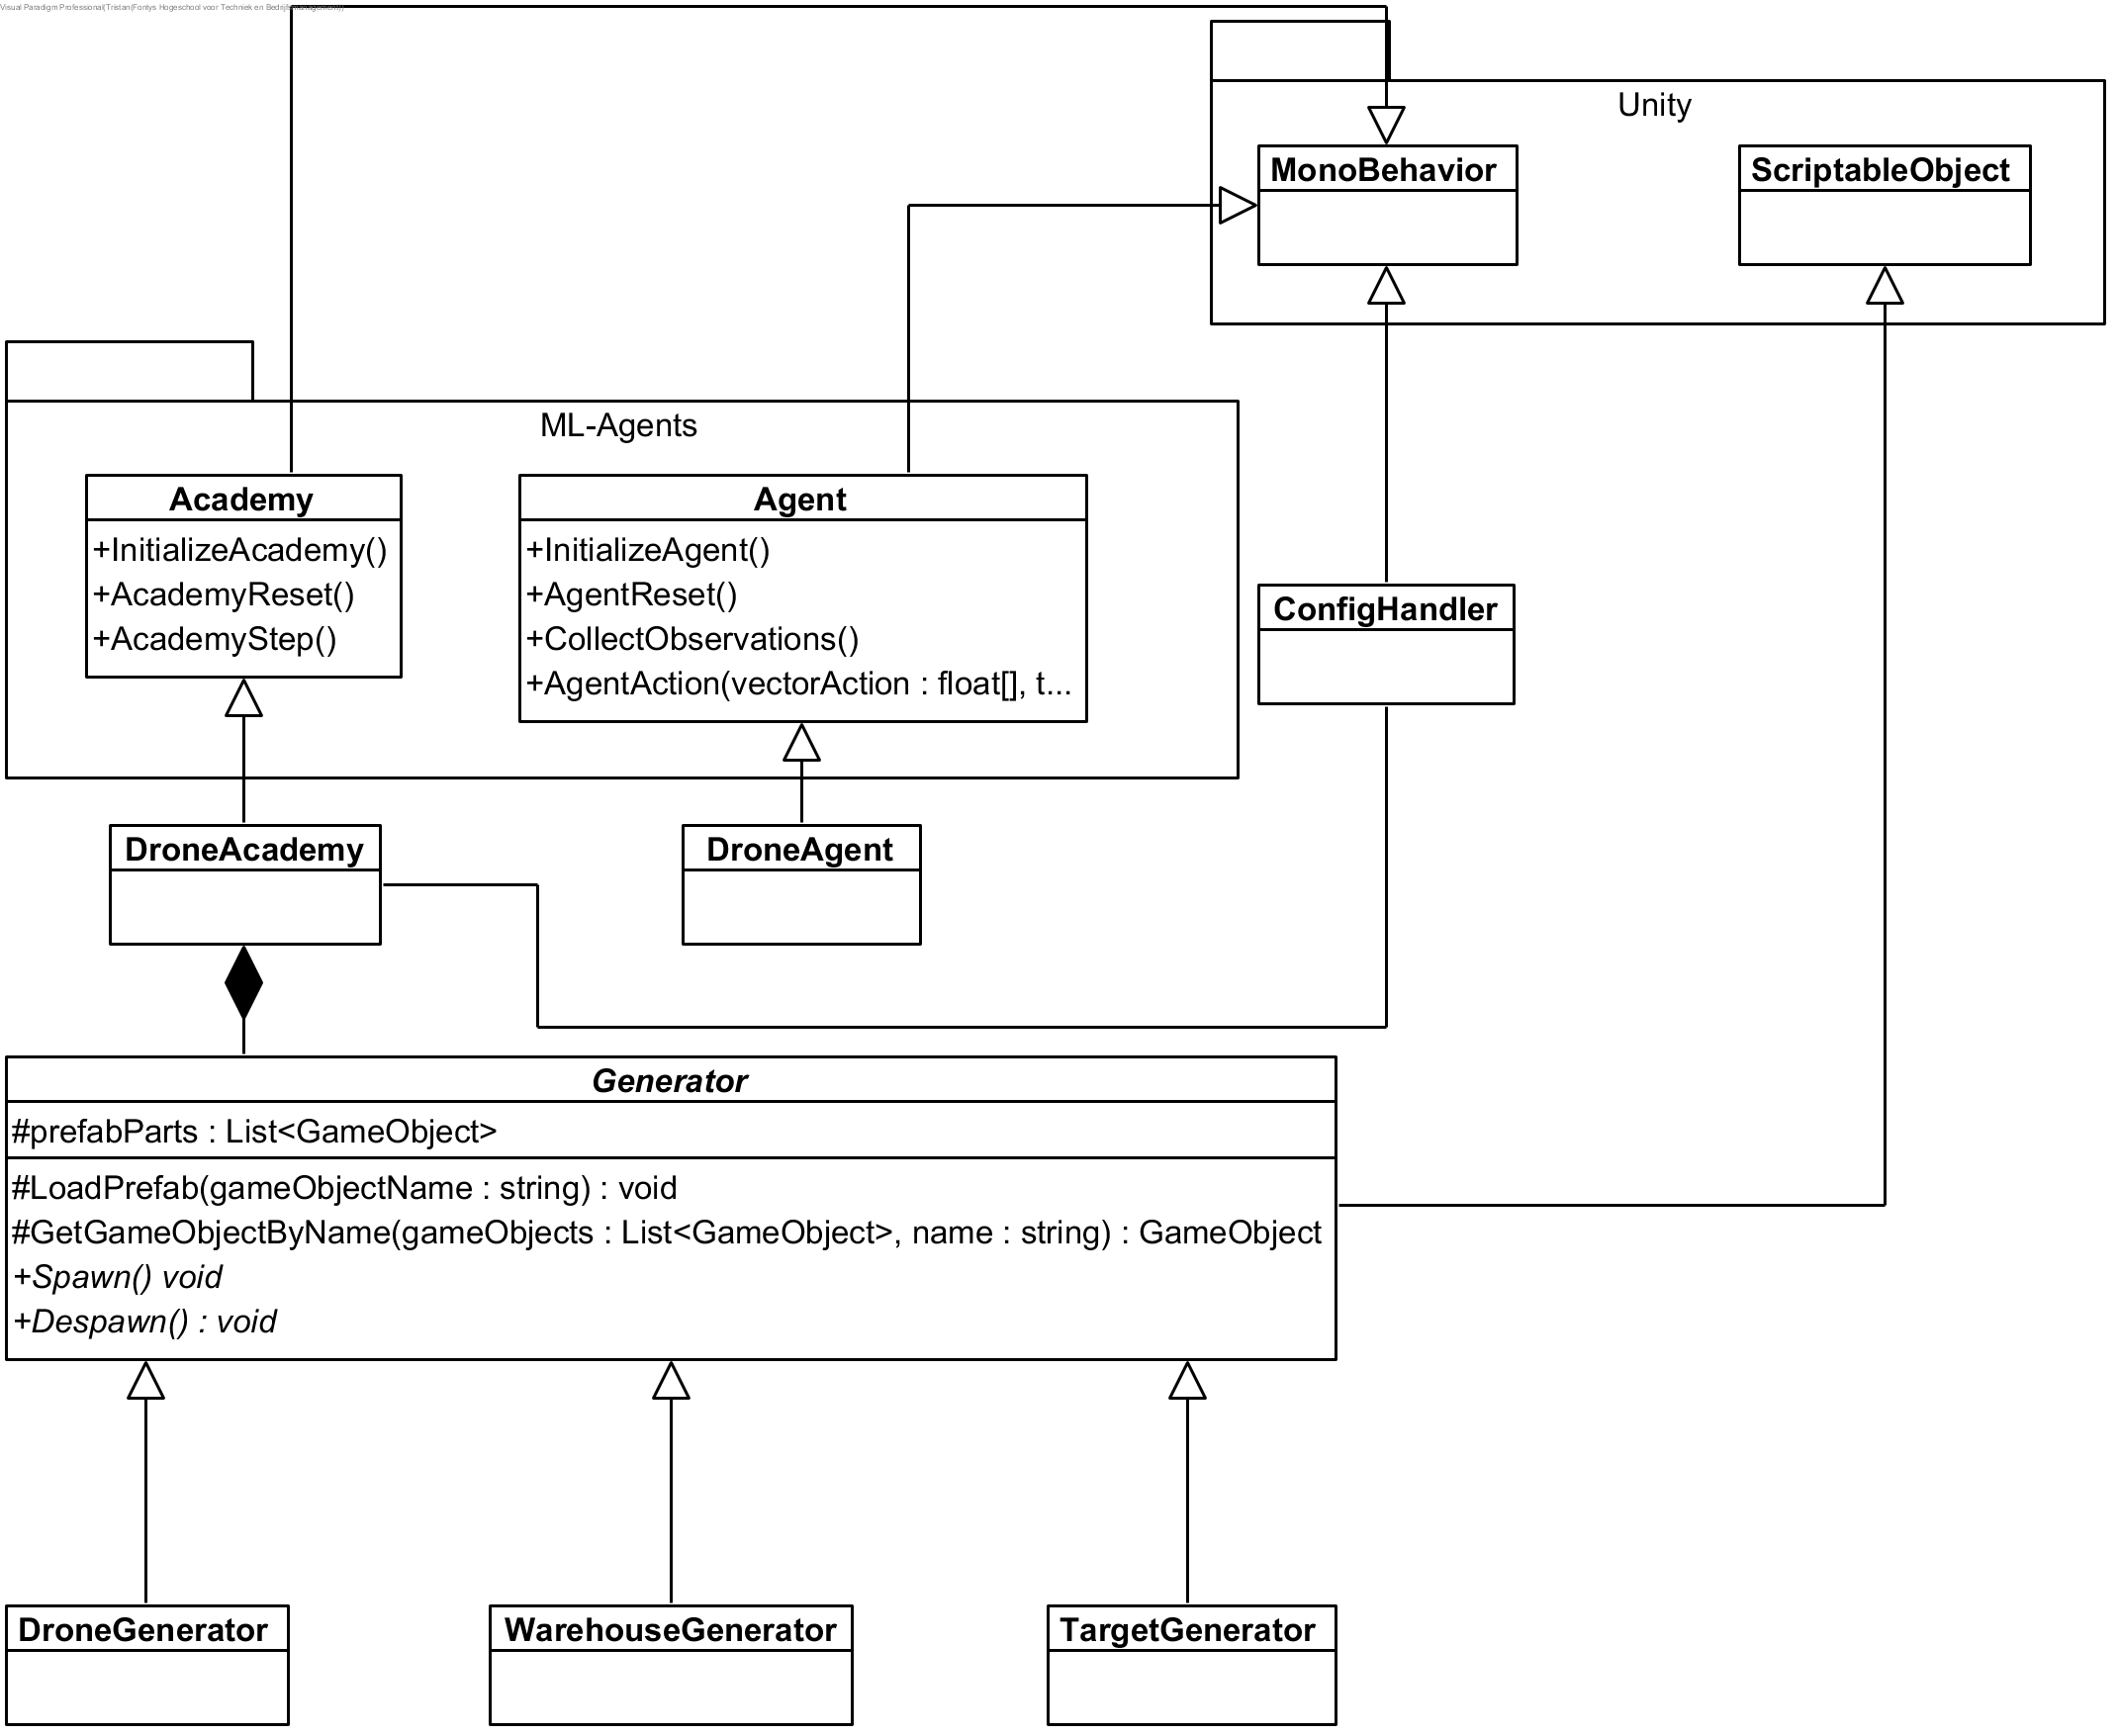
\includegraphics[width=\linewidth, angle=-90]{img/simulation_class_diagram}
	\label{fig:class_diagram}
	\caption{Partial class diagram of the code behind the simulation.}
\end{figure}
		\chapter{Setup State Machine Concept}
\lhead{\thechapter \space Setup State Machine Concept}
\label{app:setup}
This chapter provides a set of instructions to install and set up the state machine concept. The link to the Git repository has been left out as it private. The project was developed using Python 3.6.9, which is also needed to run the project.

\begin{enumerate}
	\itemsep0em
	\item Clone the repository to a local machine
	\item Switch to branch "heuristic"
	\item The project resides in the ./Python
	\item Turn on the Tello drone
	\item Once it starts flashing a green light, connect to the drone's WI-FI network.
	\item Run the file Main.py using the command "python Main.py" in the command line.
	\item Press the tab key to launch the drone, and press the "M" key to start the state machine. Note: make sure it is facing the beam before pressing "M".
	\item To stop the state machine, press "M" again.
	\item To land the drone and kill the program, press ESC. To just land the drone, press backspace.
	\item Other controls for manually controlling the drone can be found in the DroneController.py file.
\end{enumerate}

This project is dependent on the following modules which can be installed through pip:
\begin{itemize}
	\item opencv-python (version 4.1.1.26) 
	\item av (version 6.2.0)
	\item tellopy (version 0.6.0)
	\item simple\_pid (version 0.2.4)
	\item pynput (version 1.4.5)
\end{itemize}
		\chapter{First State Machine Design for Concept 2}
\lhead{\thechapter \space First State Machine Design for Concept 2}
\label{app:bar_states_simple}
\begin{figure}[h]
	\centering
	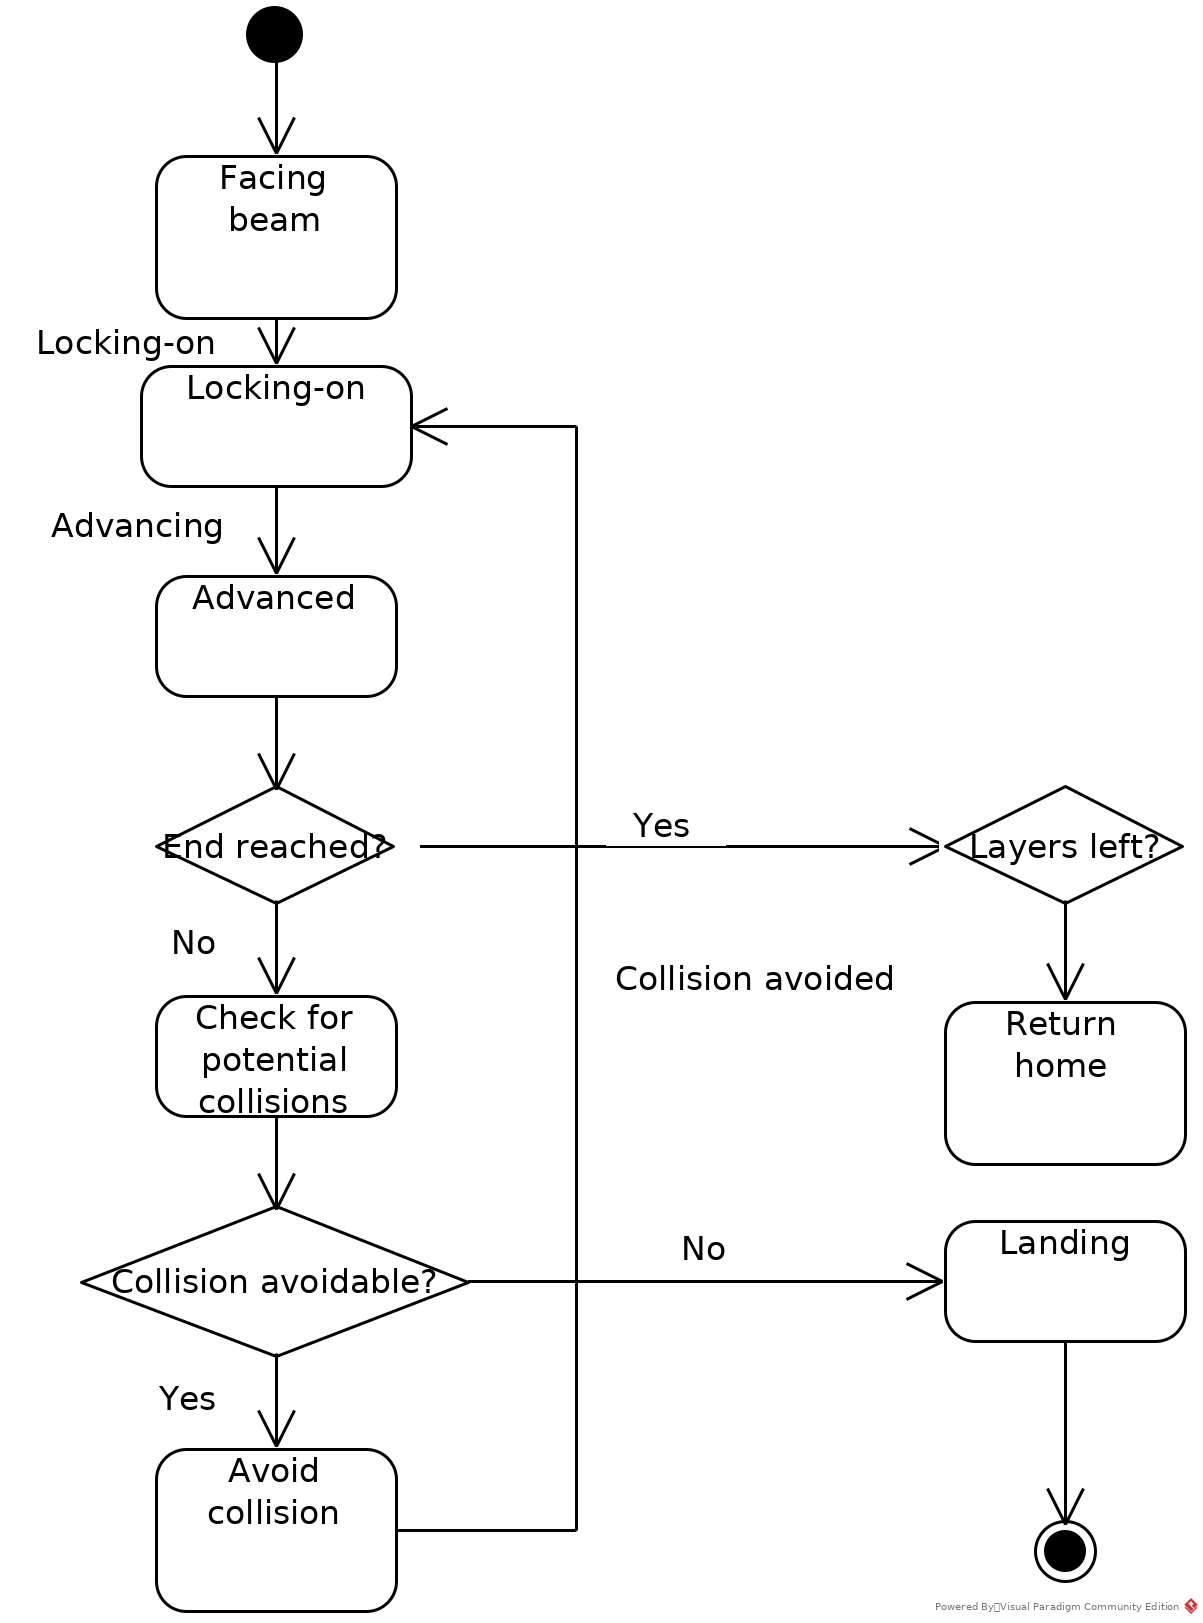
\includegraphics[height=0.6\textheight]{img/Bar_following_states_simple}
	\label{fig:bar_states_simple}
	\caption{First state diagram design for state machine concept.}
\end{figure}
		\chapter{Second State Machine Design for Concept 2}
\lhead{\thechapter \space Second State Machine Design for Concept 2}
\label{app:bar_states_two}
\begin{figure}[h]
	\centering
	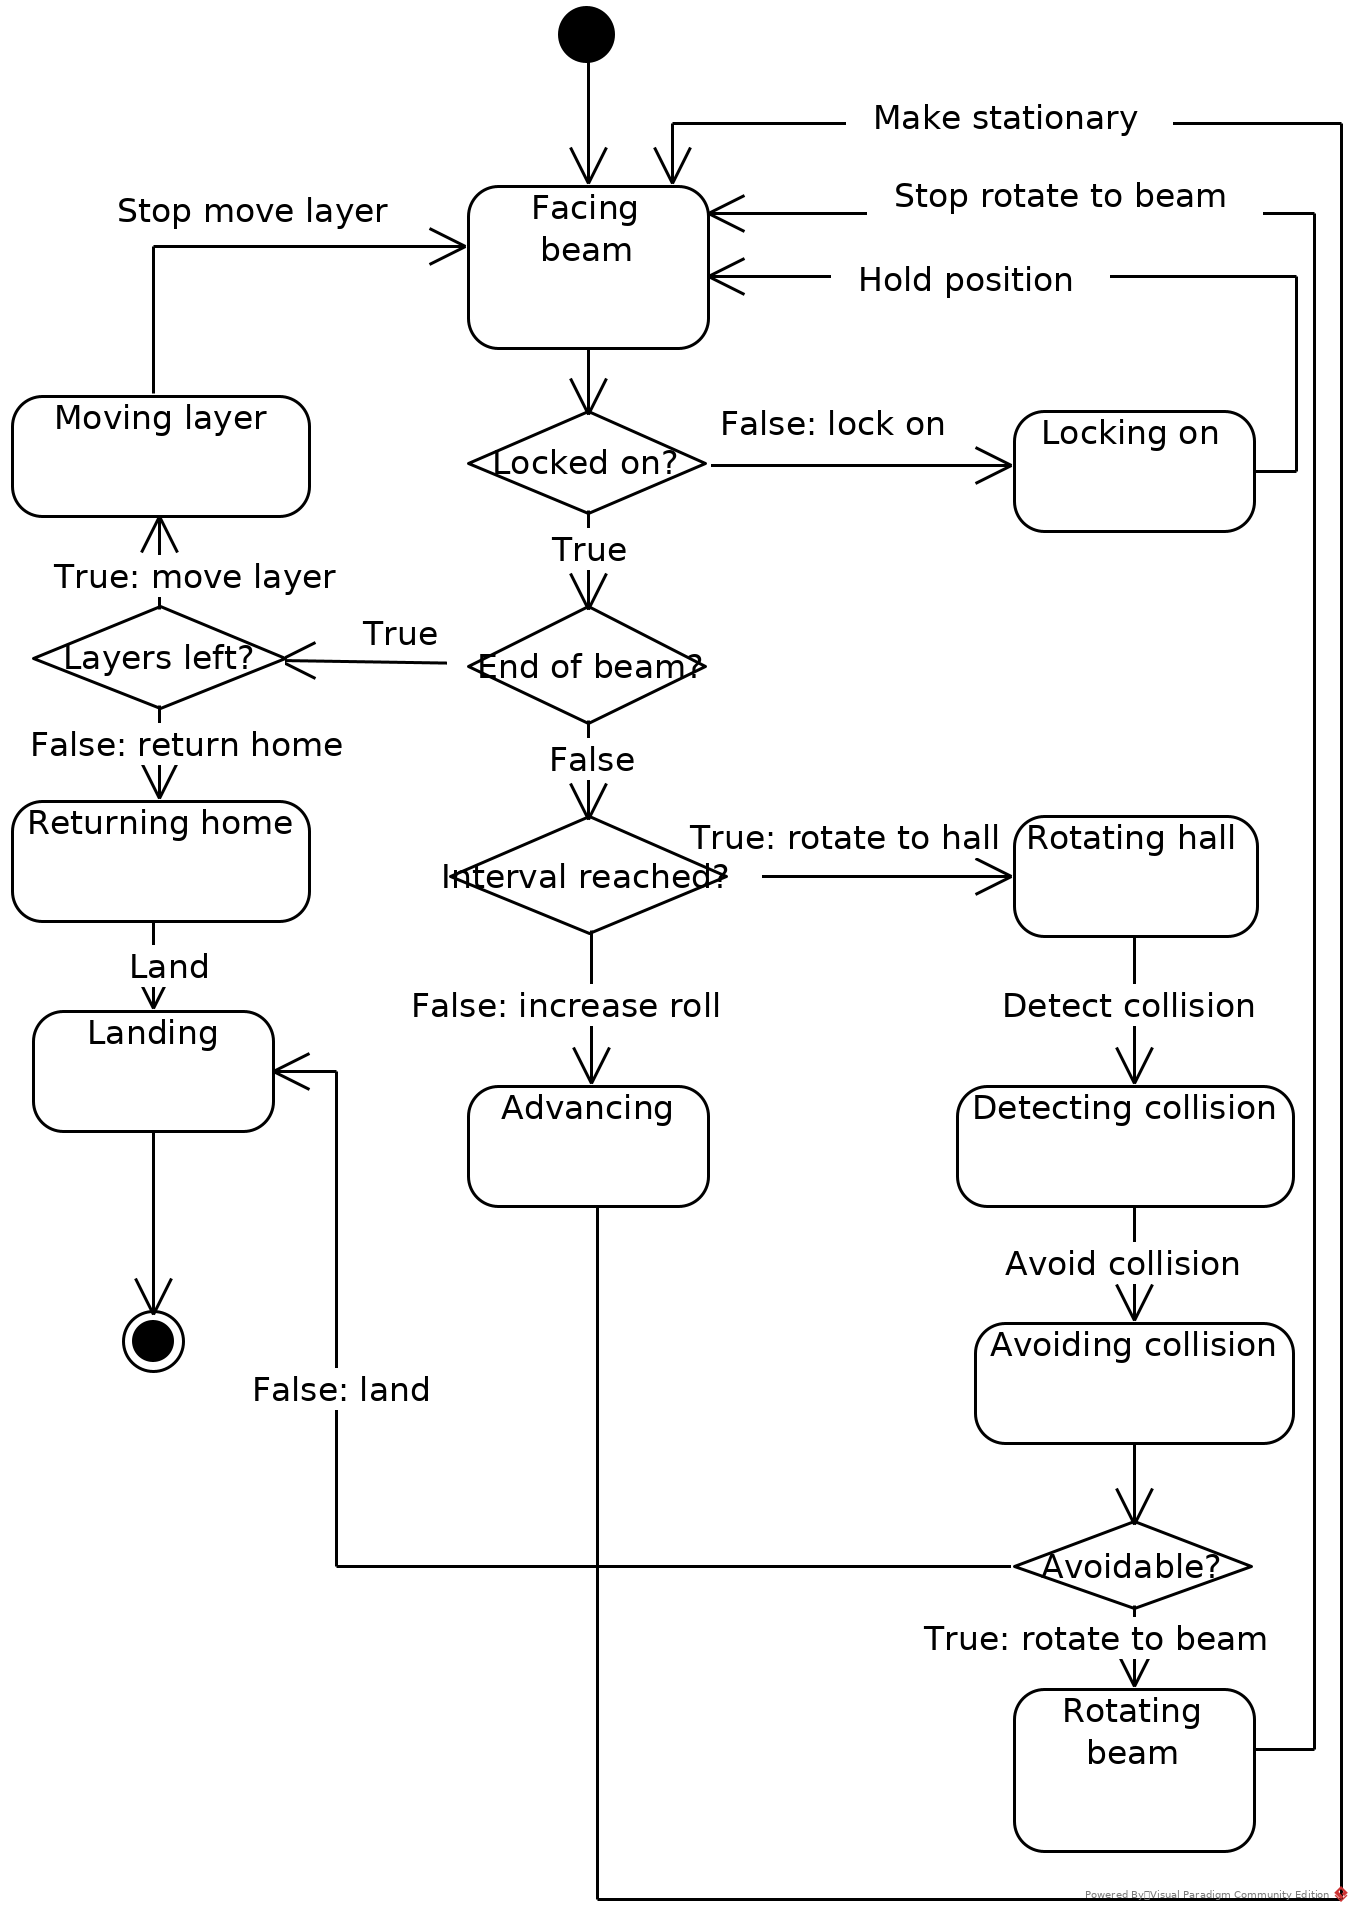
\includegraphics[height=0.6\textheight]{img/Bar_following_state_machine}
	\label{fig:bar_states_two}
	\caption{Second state diagram design for state machine concept.}
\end{figure}
		
		\chapter{Software Requirements Specification}
		Page left intentionally blank to act as cover page.
		\label{app:srs}
		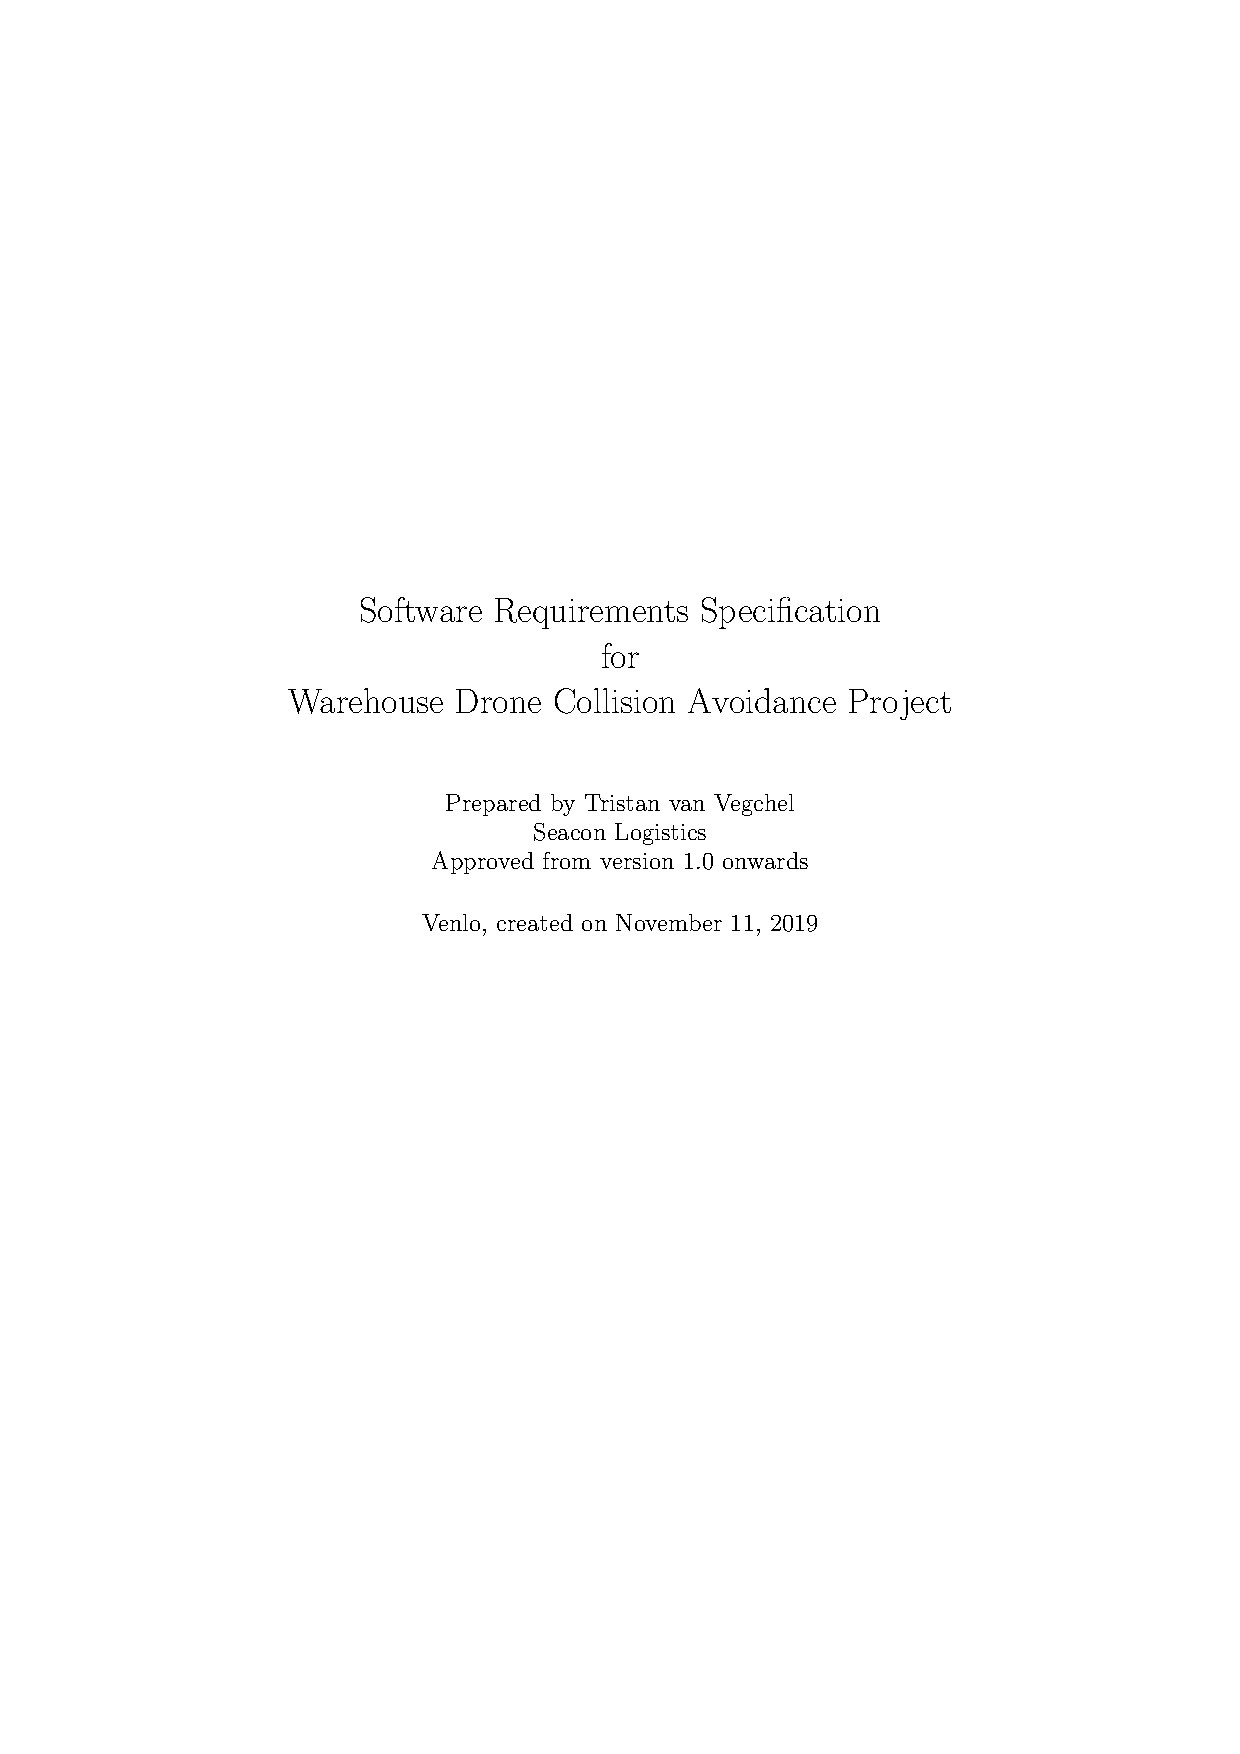
\includepdf[pages=-]{utility/SRS/SRS_warehouse_collision_avoidance}
	\end{appendices}
\end{document}